\documentclass[12pt]{article}%设置文档类型
\usepackage{geometry}%设置页面尺寸、页边距、页眉页脚的宏包
\geometry{left=1in,right=0.75in,top=1in,bottom=1in}%设置页边距宏包

\newcommand{\Problem}{C}%新命令宏包
\newcommand{\Team}{2409859}

\usepackage[table]{xcolor}

\usepackage{newtxtext}%设置英文字体
\usepackage{amsmath,amssymb,amsthm}%数学公式宏包
\usepackage{lipsum}%随机生成段落宏包
\usepackage{multirow,booktabs} %插入表格

\usepackage{float}%浮动体宏包
\usepackage{listings} % 代码宏包
\usepackage{xcolor}  % 颜色宏包
\usepackage[toc,page]{appendix} % 参考文献宏包
\usepackage[nottoc]{tocbibind}%参考文献放入目录中的宏包
\usepackage{indentfirst}%首行缩进宏包

\usepackage[pdftex]{graphicx}%插图红包
\usepackage{fancyhdr}%设置页眉页脚格式,令页眉页脚左对齐、右对齐、居中的宏包
\lhead{Team \#\Team}%控制编号宏包
\cfoot{}%清除页码
\setlength{\headheight}{15pt}%高度设置宏包
\usepackage[hidelinks]{hyperref}%让生成的文章目录有链接,点击时会自动跳转到该章节

%这里是新加的宏包
\usepackage{subfigure}
\usepackage{pdfpages}
\usepackage{longtable}
\usepackage{tabu}
\usepackage{threeparttable}
\usepackage{paralist}
\usepackage{setspace}

\usepackage{booktabs} % For better table lines
\usepackage{tabularx} % For adjustable-width columns

\usepackage{hyperref}
\hypersetup{hidelinks,
	colorlinks=true,
	allcolors=black,
	pdfstartview=Fit,
	breaklinks=true}
\usepackage{graphicx}
\let\itemize\compactitem
\let\enditemize\endcompactitem

%多行三线表
\usepackage{multirow}

\usepackage{makecell}
\usepackage{longtable}
\usepackage{booktabs}

\usepackage{lastpage} 
%表格颜色

% 信件/备忘录环境
\newcounter{prefix}  % 创建隐藏前缀计数器,避免对 letter 环境编号
\renewcommand{\theHsection}{\theprefix.\thesection}  % 针对 hyperref
\newenvironment{letter}[1]{\refstepcounter{section}\addtocounter{section}{-1}\section*{#1}\addcontentsline{toc}{section}{#1}}{\stepcounter{prefix}}
%%%%%%%%%%%%%%%%%%%%%%%%%%%%%%%%
\usepackage{appendix}


\begin{document}
	\graphicspath{{.}}  % Place your graphic files in the same directory as your main document
	\DeclareGraphicsExtensions{.pdf, .jpg, .tif, .png}
	\thispagestyle{empty}
	\vspace*{-16ex}
	\centerline{\begin{tabular}{*3{c}}
			\parbox[t]{0.3\linewidth}{\begin{center}\textbf{Problem Chosen}\\ \Large \textcolor{red}{\Problem}\end{center}}
			& \parbox[t]{0.3\linewidth}{\begin{center}\textbf{2024\\ MCM/ICM\\ Summary Sheet}\end{center}}
			& \parbox[t]{0.3\linewidth}{\begin{center}\textbf{Team Control Number}\\ \Large \textcolor{red}{\Team}\end{center}}	\\
			\hline
	\end{tabular}}
	%%%%%%%%%%% Begin Summary %%%%%%%%%%%
	% Enter your summary here replacing the (red) text
	% Replace the text from here ...
	%标题
	\begin{center}
		\LARGE {A Glimpse of Music Change through Influence Networks}
		\vspace{0.4cm}
		
		\normalsize\textbf{Summary}
	\end{center}
	
	
	% (Need to be reviewed)
	In the captivating 2023 Wimbledon Gentlemen’s final, the tennis world witnessed an extraordinary display of skill, resilience, and strategic mastery as 20-year-old Spanish sensation Carlos Alcaraz overcame the formidable Novak Djokovic, a seasoned champion with an illustrious career. 
	
For Task 1, to assess the performance of players on the field, we employed \textbf{PCA} (Principal Component Analysis) to perform dimensionality reduction on the raw data. Six indicators with the most informative content were extracted from the data. Subsequently, the \textbf{WME} (Weighted Maximum Entropy) entropy weighting method was applied to assign appropriate weights, thus achieving a quantitative evaluation of performance. In the end, we obtained the distribution of visual performance scores for Djokovic and opponents in a match, as illustrated in Figure \ref{r3}.

For Task 2, building upon a performance-based model, we introduced the concept of "momentum." To verify the randomness of momentum fluctuations, we utilized a \textbf{run test algorithm}, and the results are presented in Table \ref{22222}. According to the test results, it was evident that the fluctuations were not random.

For Task 3,  To predict momentum fluctuations in tennis matches, based on the provided Wimbledon tennis data, we constructed \textbf{GSRF} (Grid Search Random Forest) and \textbf{GRFA} (Grid Random Forest Algorithm) models to forecast momentum fluctuations for the 2023 Wimbledon tennis competition. Subsequently, based on differences in momentum fluctuations, we defined turning points in the course of the matches, employing the \textbf{CUMSUM} algorithm to identify transitions in the trend of winning or losing. Finally, we utilized the predicted tennis match data and the identified turning points within the matches to offer corresponding recommendations to the players.

Furthermore, we employed three evaluation metrics: RMSE (Root Mean Square Error), MAE (Mean Absolute Error), and MAPE (Mean Absolute Percentage Error) to assess the predictive performance of the two models. Through a comparative analysis of the MAPE values of the two models, we found that the GSRF (Grid Search Random Forest) prediction model exhibited superior predictive performance. We selected one metric for sensitivity analysis and introduced Gaussian noise into the GSRF model parameters for stability testing.

Regarding the fourth question, we observed that the GSRF model demonstrated notable predictive performance when handling multi-scenario data. When applied to the 2023 Wimbledon women's tennis match data, it also exhibited strong predictive results. These findings provide some evidence for the versatility of the GSRF model.

	Finally, we discuss the advantages and disadvantages of the model and make some scientific-based suggestions for coaches. 
	
	% Here is the abstract of your paper.
	
	% Firstly, that is ...
	
	% Secondly, that is ...
	
	% Finally, that is ...
	
	% 美赛论文中无需注明关键字。若您一定要使用,
	% 请将以下两行的注释号 '%' 去除,以使其生效
	\vspace{5pt}
	\textbf{Keywords}: GSRF model, PCA, WME, GRFA, CUMSUM algorithm, Evolutionary factors
	
	
	
	\clearpage%另起一页
	\pagestyle{fancy}
	% Uncomment the next line to generate a Table of Contents
	%\tableofcontents 
	\newpage
	\thispagestyle{empty}
	\rhead{Page \thepage~of~\pageref{LastPage}}
	
	%%%%%%%%%%%%%%%%%%%%%%%%%%%%%%
	%目录 
	\begin{center}
		\tableofcontents
	\end{center}		
	\newpage
	
	\section{Introduction}
	
	\subsection{Background}
The unpredictability of sports was fully demonstrated in the 2023 Wimbledon Wimbledon Gentlemen’s final. The match between the young Spanish player Carlos Alcaraz and the experienced Novak Djokovic was not only a contest of technique and stamina but also a battle of psychology and the shifts in "momentum." \cite{gollub2019producing} During different stages of the match, both players experienced fluctuations in momentum. Especially at critical moments, the momentum seemed to be able to affect \cite{sipko2015machine} the direction of the match and even change the outcome. \\

\begin{figure}[H]
	\centering
	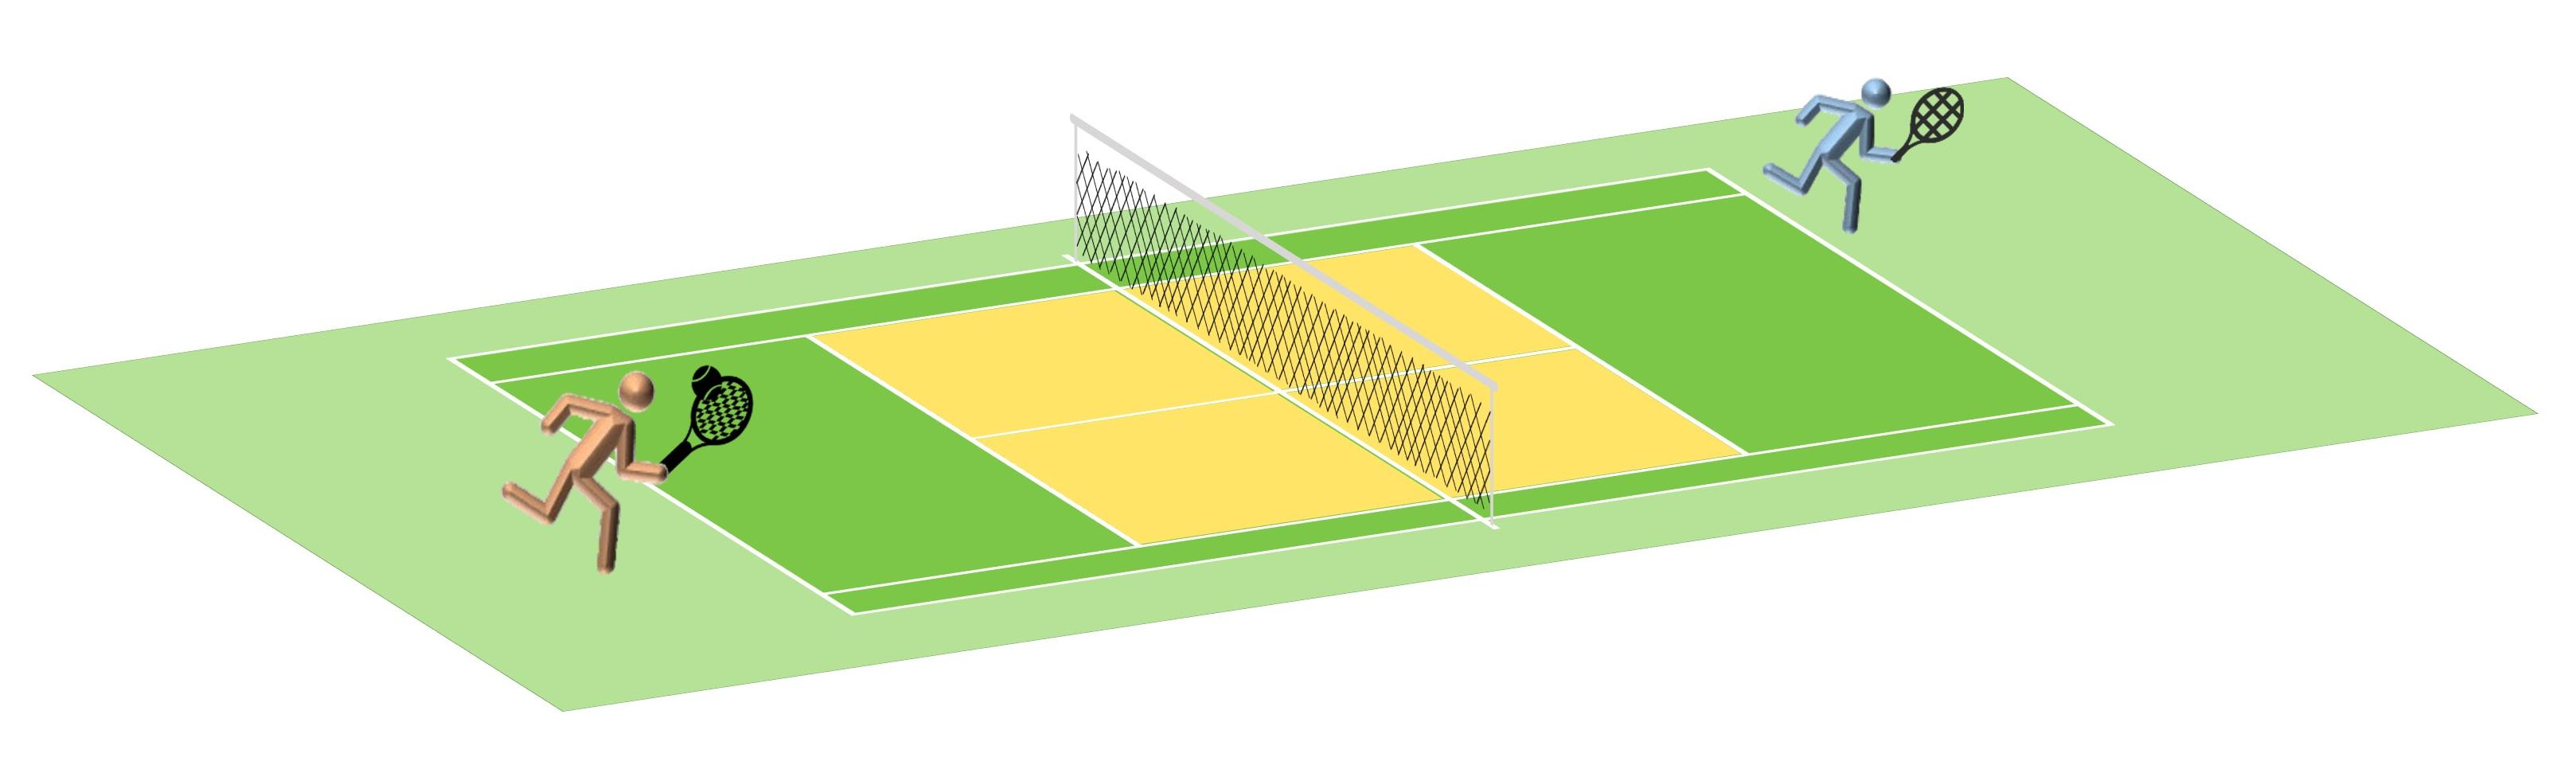
\includegraphics[scale=0.35]{figure//pp.jpg}
	\label{pp}
\end{figure}



	
	\subsection{Problem Restatement}
Considering the background information, we summarize the tasks that need to be addressed as follows:
	\begin{itemize}
		\setlength{\parsep}{0ex} %段落间距
		\setlength{\topsep}{2ex} %列表到上下文的垂直距离
		\setlength{\itemsep}{1ex} %条目间距
		\item \textbf{Task 1:} Construct a model to capture the flow of the match at the time of scoring.
		
		\item \textbf{Task 2:} Use the model to evaluate whether "momentum" has significance in the match.
		
		\item \textbf{Task 3:} Determine the key indicators that impact the game and use them to predict future fluctuations in matches.
		
		\item \textbf{Task 4:} Analyze the "momentum" differences in past matches and offer some tactical suggestions for the players. 
		
		\item \textbf{Task 5:} Test our match fluctuation prediction model and analyze its generalizability. 
		
	\end{itemize}
	
\clearpage
	\subsection{Our work}

Considering the background and the problems, our work mainly includes the following:	
\begin{figure}[H]
	\centering
	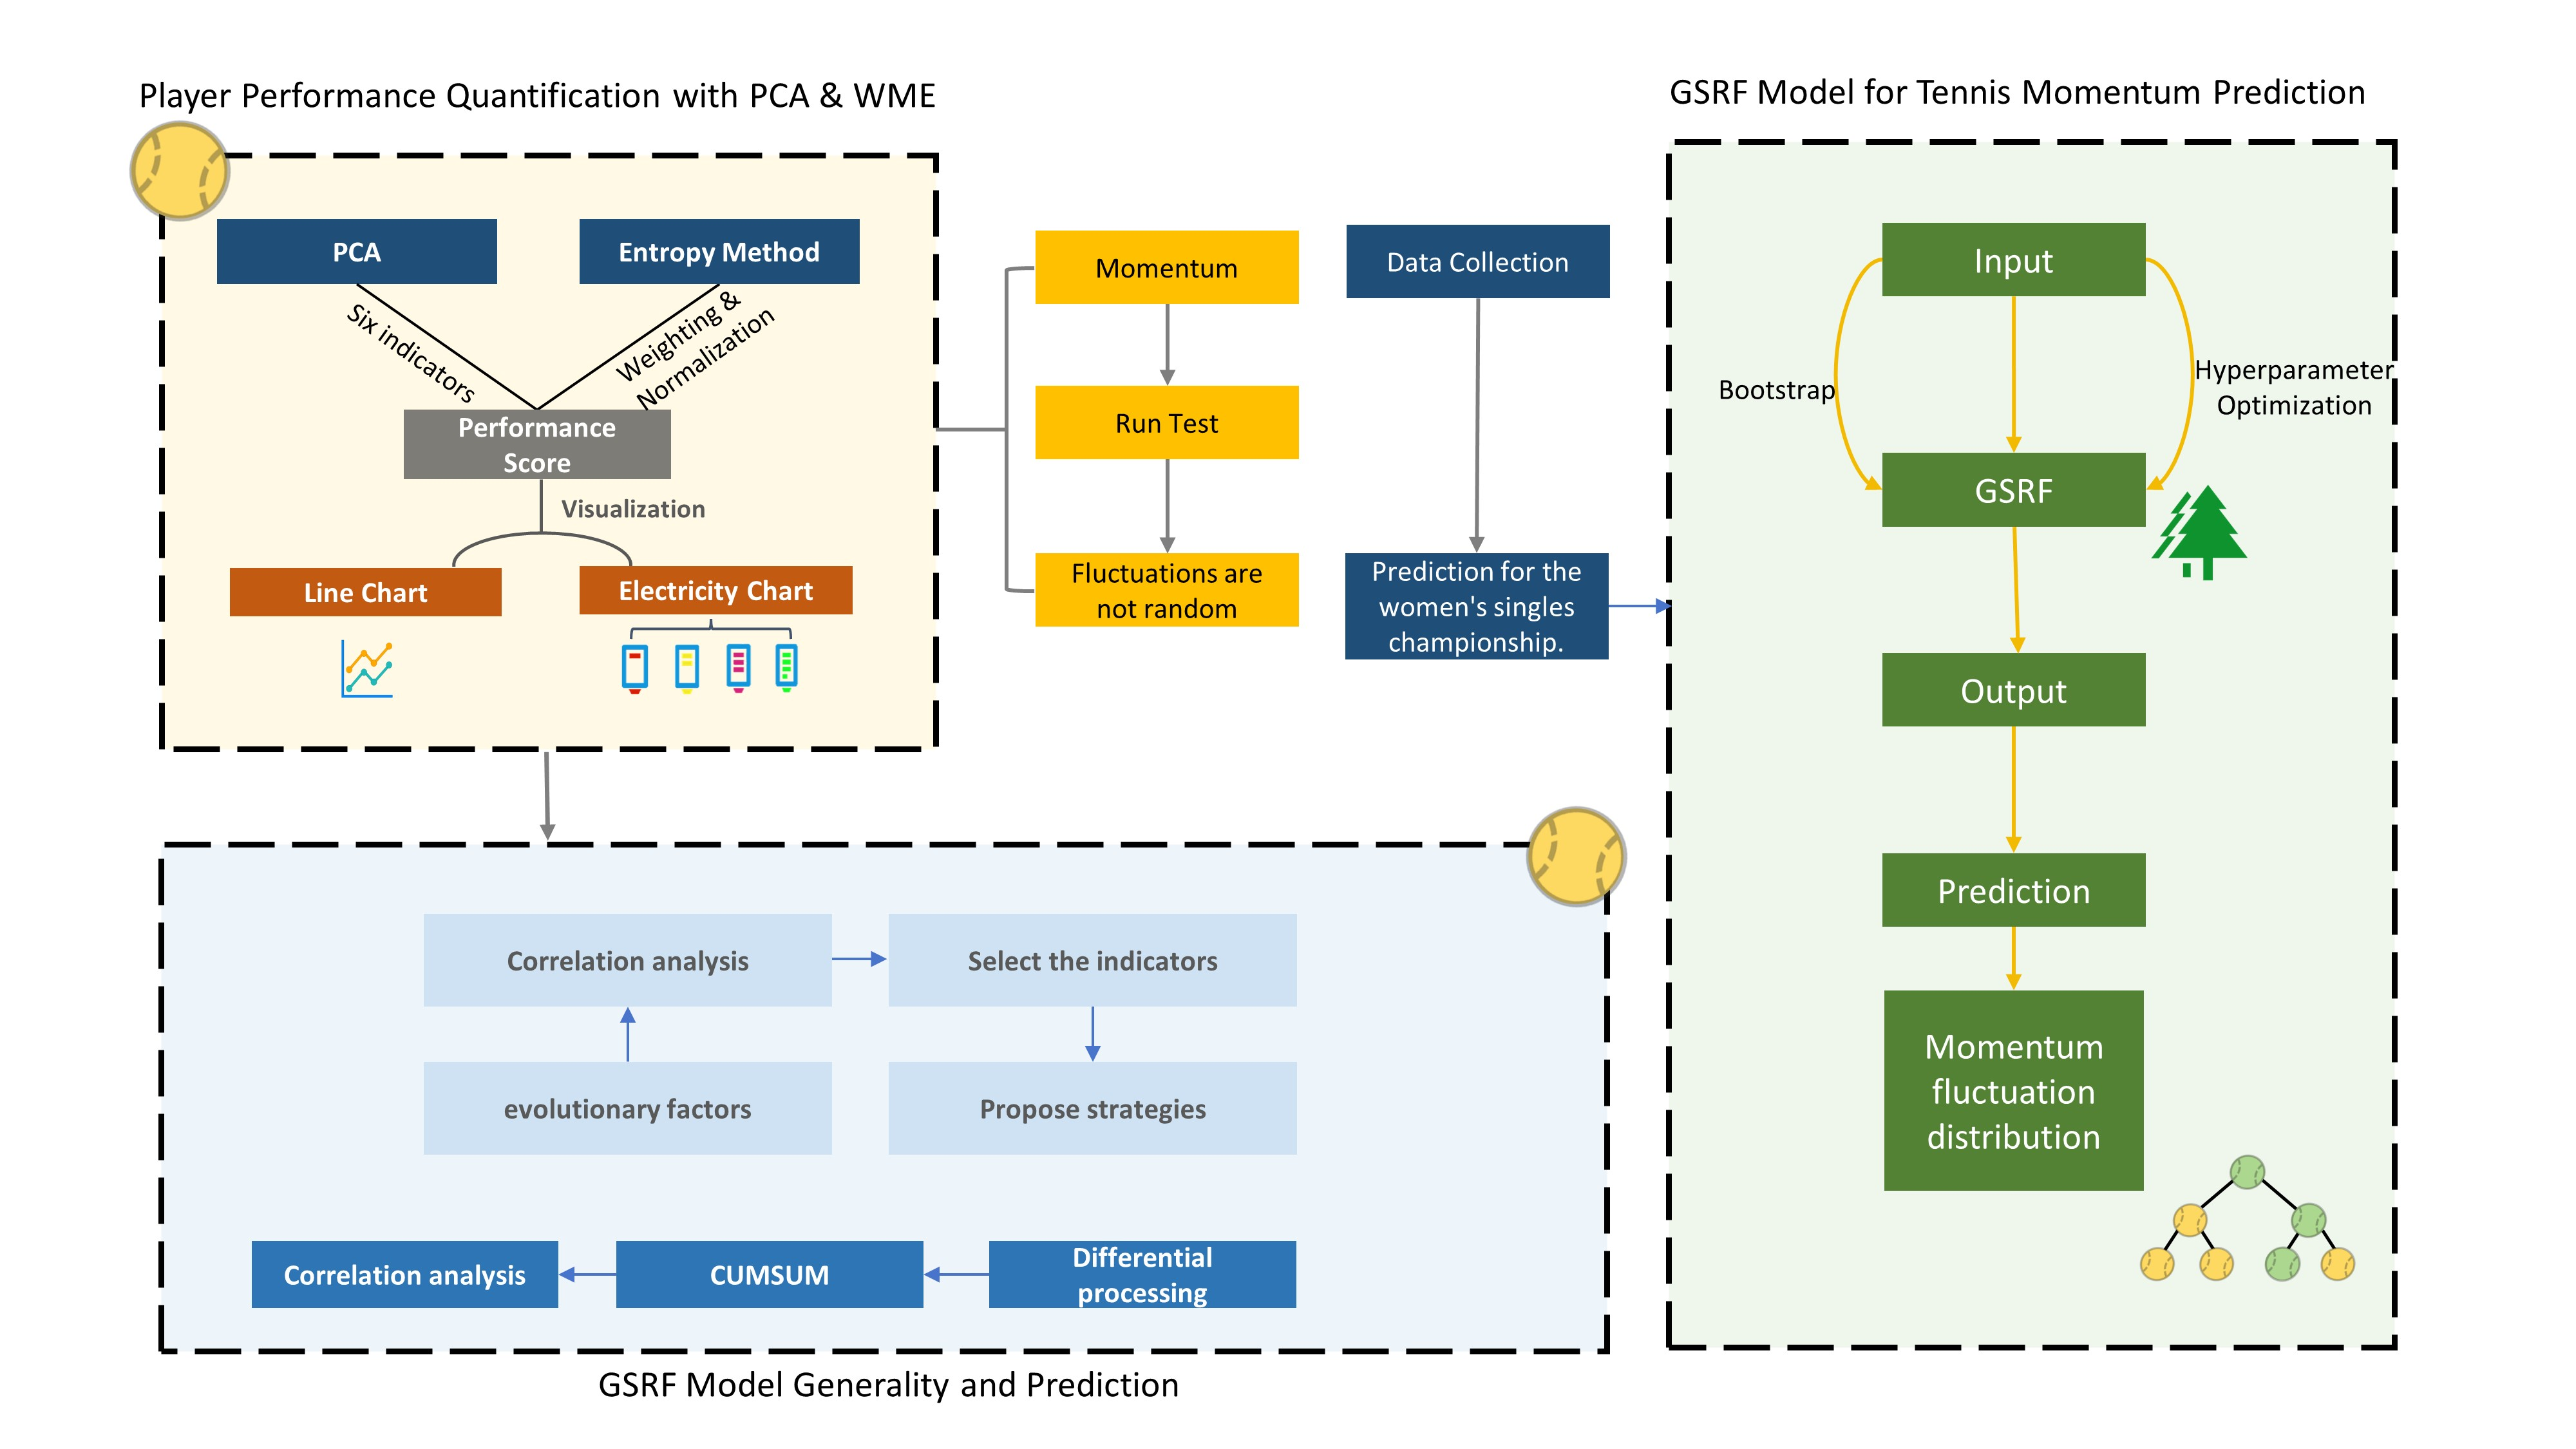
\includegraphics[scale=0.54]{figure//work.jpg}
		\caption{Our work}
	\label{11111}
\end{figure}

	
	\section{ Model Preparation}
	\subsection{Notations}
	\begin{table}[H]
		\centering
		\caption{Notations Table}
		\begin{tabular}{ll}
			\hline
			\hline
			\rowcolor{black!20}
			\multicolumn{1}{c}{\textbf{Notations}} & \textbf{Definition}\\ \hline
			$Z_x$                      & The statistical measure                   \\
			\rowcolor{black!8}
			$G_x$                      & the indirect influence from n to n+1                      \\
			$\hat{Y_i}$                       & the attenuation degree of the influence                      \\
			\rowcolor{black!8}
			$D(t)$                      & Differential sequence                       \\
			$F(t)$                      & the music influence of $i$                      \\
			\rowcolor{black!8}
			$G(t)$                      &     Represents the momentum value         \\
		
			$\psi _(t)$                      & Activity changes with time                     \\
				\rowcolor{black!8}
			$Y_i$                      & actual observed value  \\                     
			\hline
			\hline
		\end{tabular}
	\end{table}
	
	\subsection{Assumptions and Justifications}
	To simplify the problem, we make the following basic assumptions: \\
	\begin{itemize}
		\setlength{\parsep}{0ex} %段落间距
		\setlength{\topsep}{2ex} %列表到上下文的垂直距离
		\setlength{\itemsep}{1ex} %条目间距
		\item \textbf{Assumption1:} Assumes no injuries during matches.
		
		\textbf{$\hookrightarrow$Justification:} This ensures analysis isn't skewed by injuries, keeping evaluations of strategies and performance consistent and reliable.
		
		\item \textbf{Assumption2:} Excludes psychological factors.
		
		\textbf{$\hookrightarrow$Justification:} Removing psychological variables simplifies the model, allowing a focus on tangible, measurable performance indicators like skill and endurance.
		
		\item \textbf{Assumption3:} Presumes slight differences in player abilities.
		
		\textbf{$\hookrightarrow$Justification:} This approach mitigates the impact of outliers, aiming for data reliability by assuming a minimal variance in player skill levels.
		
		\item \textbf{Assumption4:} Maintains constant match rules. 
		
		\textbf{$\hookrightarrow$Justification:} Keeping match rules unchanged ensures data uniformity, allowing for accurate comparisons and analyses that reflect real-match scenarios.
	\end{itemize}
	
	
	
	
	\subsection{Data Preprocessing and Data Labeling}
	\subsubsection{Data preprocessing}
	Upon observation of the provided data, we first process following three types of data: 
		\begin{enumerate}[\bfseries 1.]
		\setlength{\parsep}{0ex} %段落间距
		\setlength{\topsep}{1ex} %列表到上下文的垂直距离
		\setlength{\itemsep}{0.6ex} %条目间距
		\item  Missing data. (1) For the missing data on match outcomes. We noticed that some match results were missing. By examining the official data of the Wimbledon tournament, we filled in these missing pieces of data. (2) For the missing data on player indicators. The "speed" column has missing data, which we have filled in with the average serve speed of the players in the current game.
		\item Non-numeric data. To facilitate the analysis of the data, we converted these data into numeric values. For example, in the player-score column, we replaced "AD" (Advantage) with the numeric data "45".
		\item Different scoring systems in the same column of data. Two different scoring systems appeared in the player-score column. We standardized the scoring system to 15, 30, 40.

	\end{enumerate}

\subsubsection{Data Labeling}
 To analyze the scoring advantage of P1 and P2 individually, we have split the point$\_$victor into two dimensions, each pointing to P1 and P2, respectively. This is to indicate whether P1 or P2 scores at that point.
	
	
	
\section{Player Performance Quantification with PCA \& WME}

In this section, we first use PCA to perform dimensionality reduction on all match indicator data to identify seed indicators; then we concentrate on the final match data and conduct a thorough analysis of the match data for Carlos Alcaraz and Novak Djokovic to explore the match flow at the time when scoring occurs.
\begin{figure}[H]
	\centering
	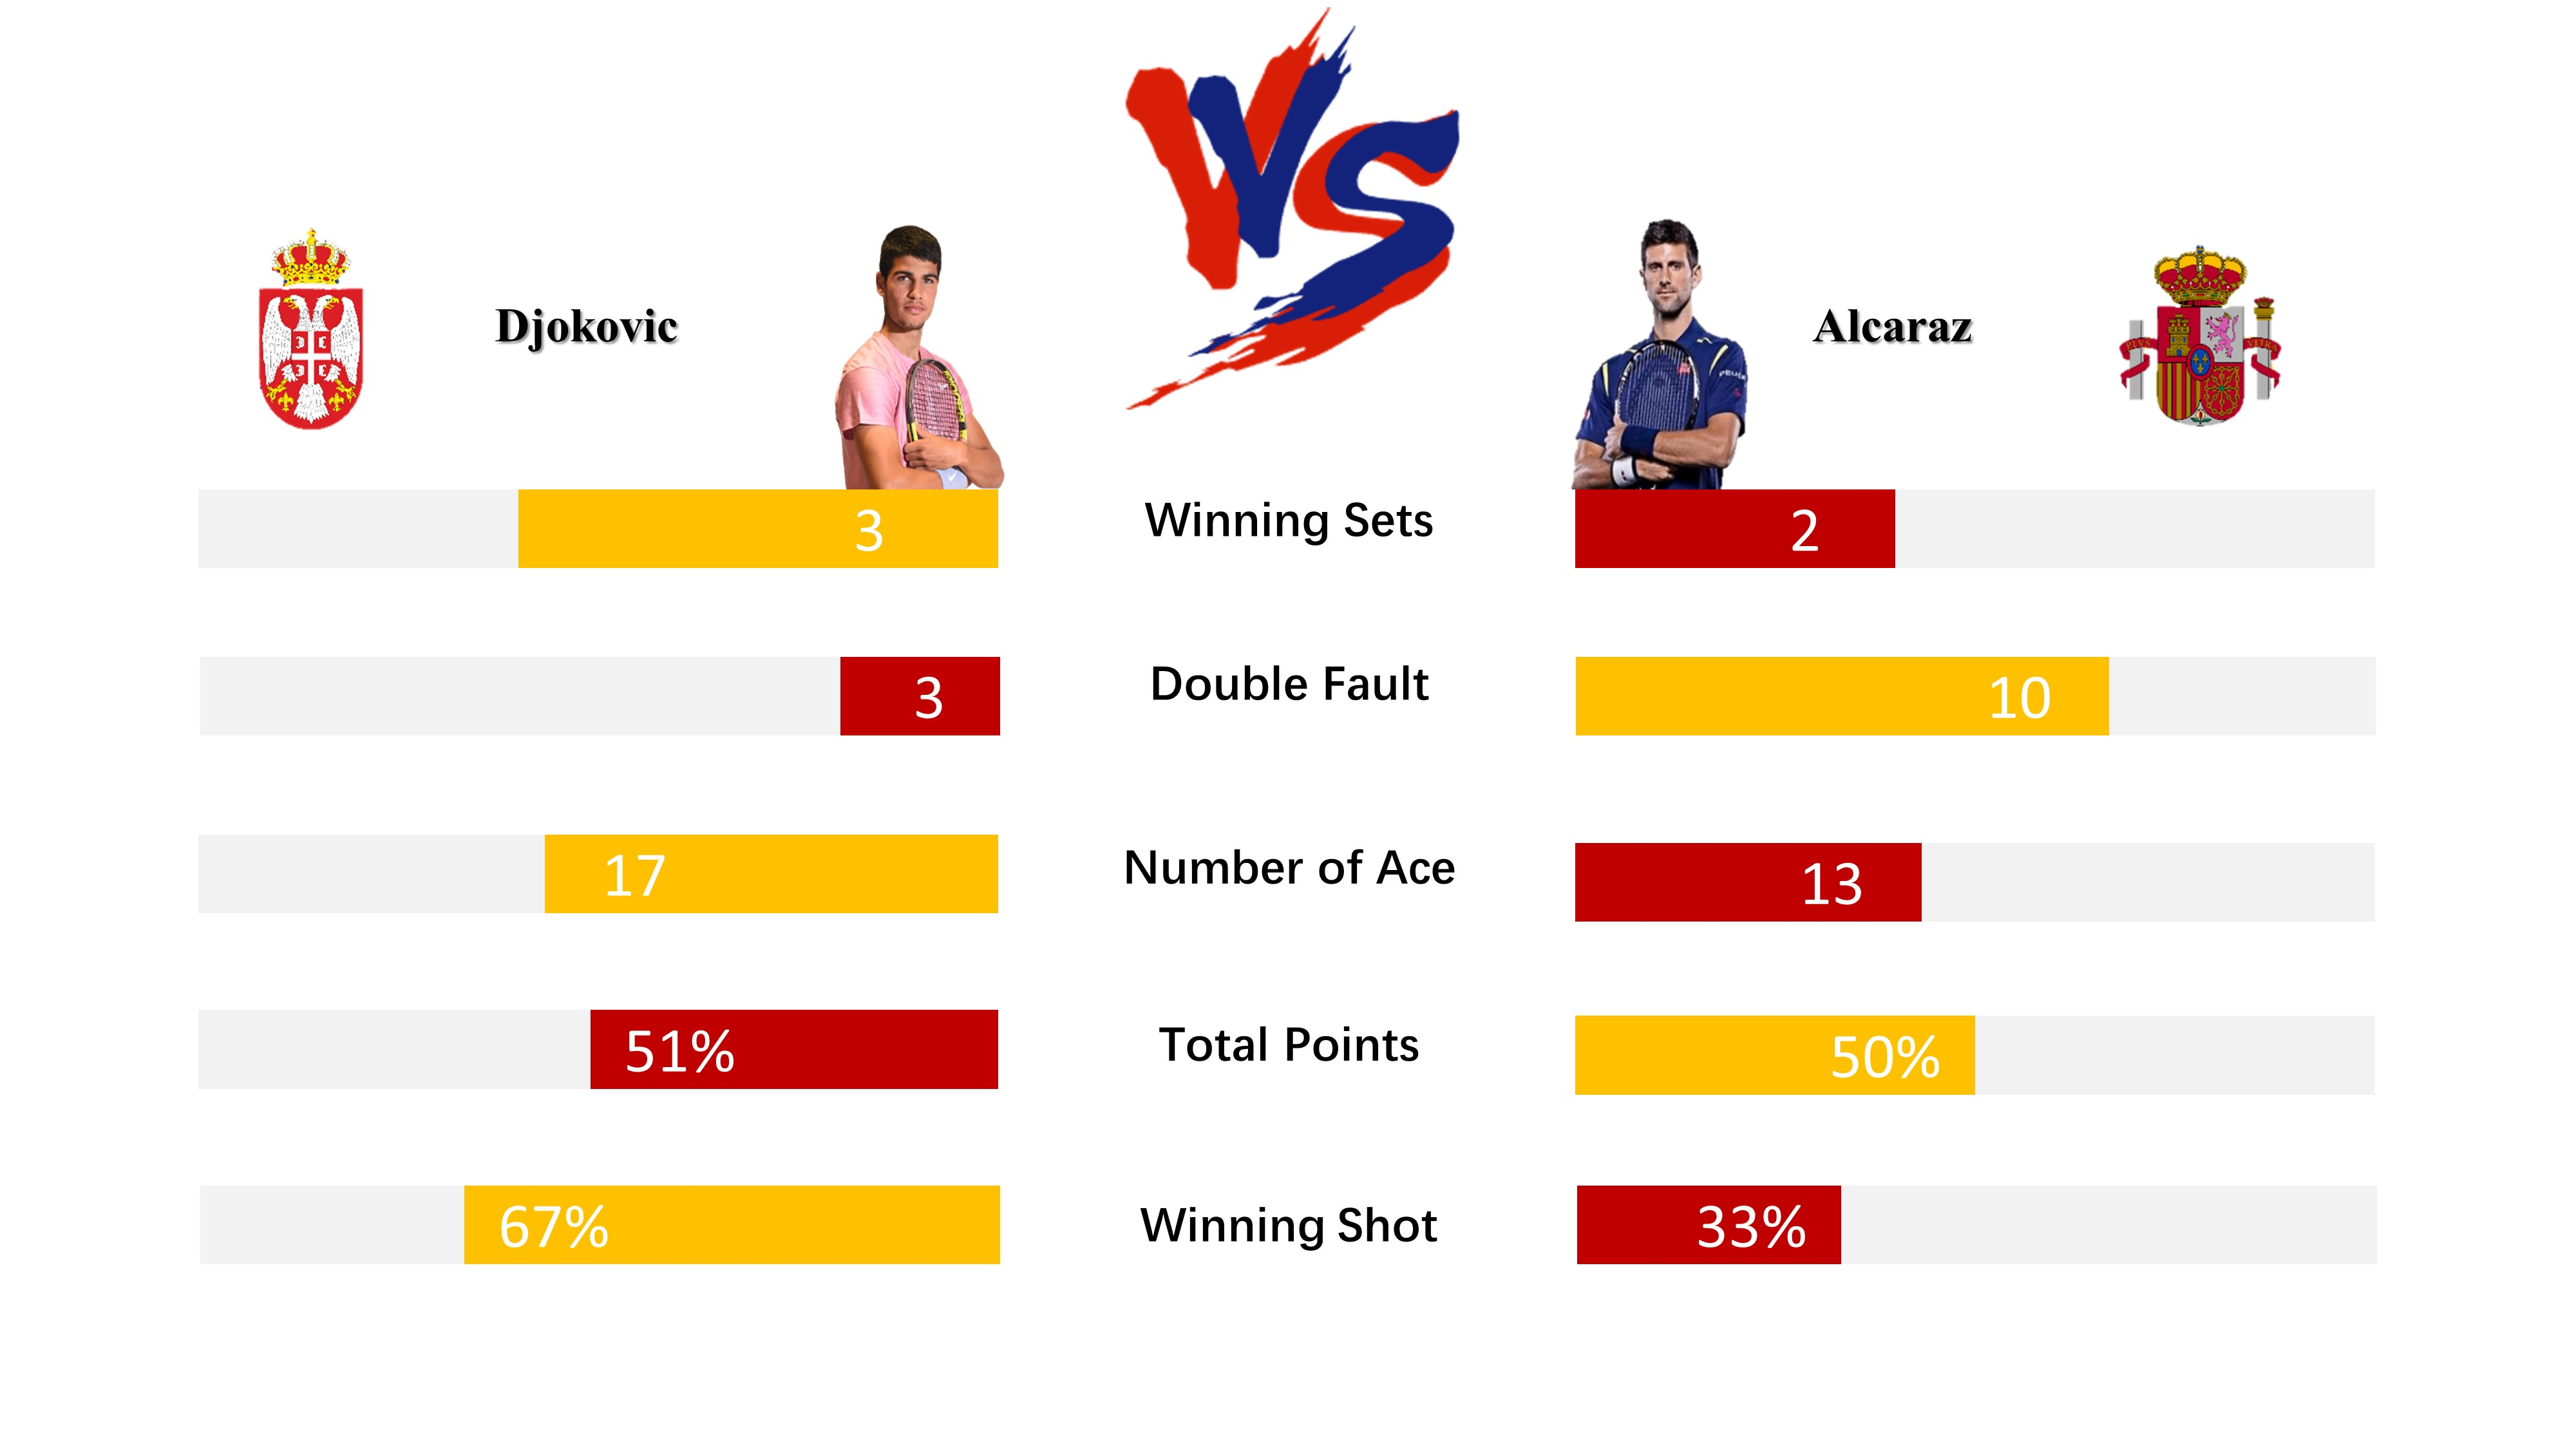
\includegraphics[scale=0.54]{figure//pk.jpg}
%%	\caption{Carlos Alcaraz VS Novak Djokovic}
	\label{pk}
\end{figure}

	
	
	\subsection{Definition of B—the Performance Score}
	
	To better quantify players' performance and scoring in the game, we propose a new definition: Performance Score, denoted as the symbol $\beta$. 
	
	\subsection{Variable Selection Based on PCA}
	
We utilized Principal Component Analysis (PCA) to analyze all match indicators \cite{yue2022study}. Through PCA, we effectively reduced the dimensionality of the data while retaining the main variables that best explain the performance of the players. The cumulative variance during the PCA process is shown in Figure \ref{pca1}.
\begin{figure}[H]
	\centering
	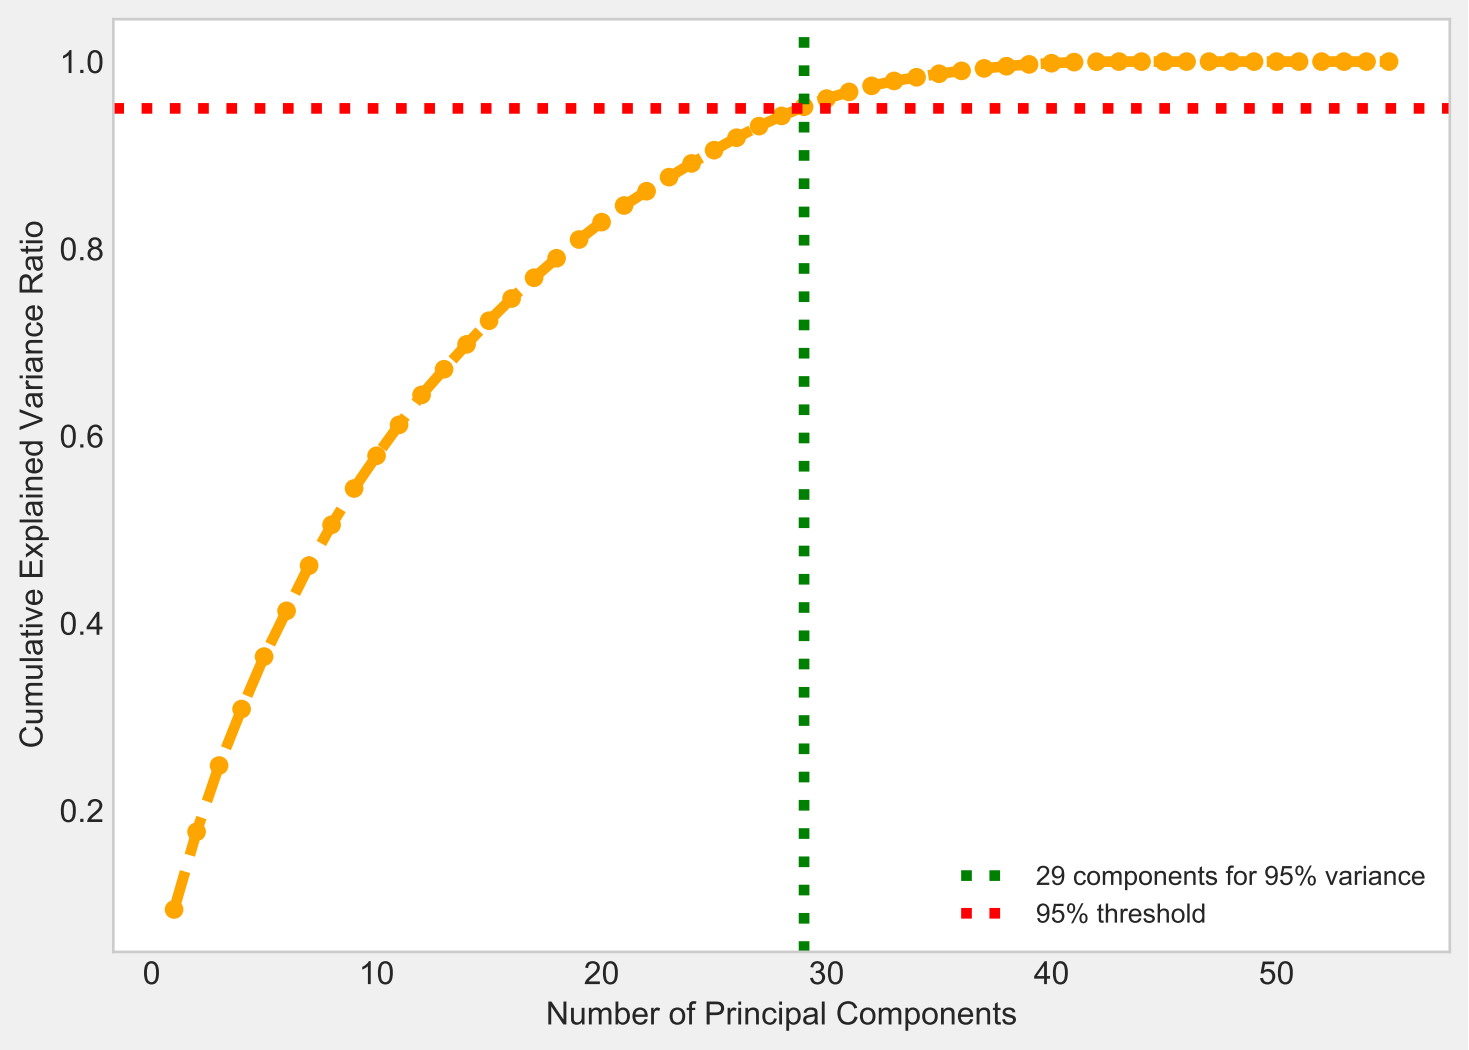
\includegraphics[scale=0.5]{figure//pca1.png}
	\caption{Explained Variance Cumulation by PCA Components}
	\label{pca1}
\end{figure}
PCA can simplify the complex dataset, allowing us to focus on the factors that have the greatest impact on match outcomes. The top 8 principal variables are presented in Table \ref{pca2}.

\begin{table}[H]
	\centering
	\caption{Top 8 principal variables}
	\begin{tabular}{cccc}

		\hline
		\hline
		\rowcolor{orange!50}
		Indicators          & PC1      & PC2       &                      \\
		\hline
		\rowcolor{yellow!30}
		p1\_ace            & 0.737698 & 0.68423   &                      \\
		\rowcolor{yellow!30}
		p1\_break\_pt\_won & 0.046219 & 0.030478  &                      \\
		\rowcolor{yellow!30}
		p1\_winner         & 0.811273 & 0.088375  &                      \\
		\rowcolor{yellow!30}
		p1\_unf\_err       & 0.24327  & 0.374712  &                      \\
		\rowcolor{yellow!30}
		p1\_net\_pt\_won   & 0.346378 & 0.665525  &                      \\
		\rowcolor{yellow!30}
		server             & 0.569129 & 0.605448  & \multicolumn{1}{l}{} \\
		\rowcolor{yellow!15}
		p1\_distance\_run  & 0.229441 & -0.266482 & \multicolumn{1}{l}{} \\
		\rowcolor{yellow!15}
		p1\_score          & 0.419781 & 0.61412   & \multicolumn{1}{l}{} \\ \hline \hline
		&          &           & \multicolumn{1}{l}{}
		\label{pca2}
	\end{tabular}
\end{table}

PC1 represents the offensive capability or scoring ability in the match, which includes service points, winners, etc.

PC2 represents the technical diversity and tactical aspects of the match, including service points, points at the net, and how to maintain high scores while reducing errors. \\

Based on Figure \ref{pca1} and Table \ref{pca2} , the top 6 indicators are selected by us as seed indicators for subsequent analysis.
\subsection{Correlation Analysis}
%Through the analysis of PCA and literature review, we extracted 6 valid indicators as seed indicators from the original data. We conducted a Spearman correlation analysis on six seed indicators for Player 1 and Player 2 respectively, as shown in Figure \ref{hot}.

\begin{figure}[H]
	\centering    
	\subfigure[For player 1]{				% 图片1([]内为子图标题)
		\label{hot1}							% 子图1的标签
		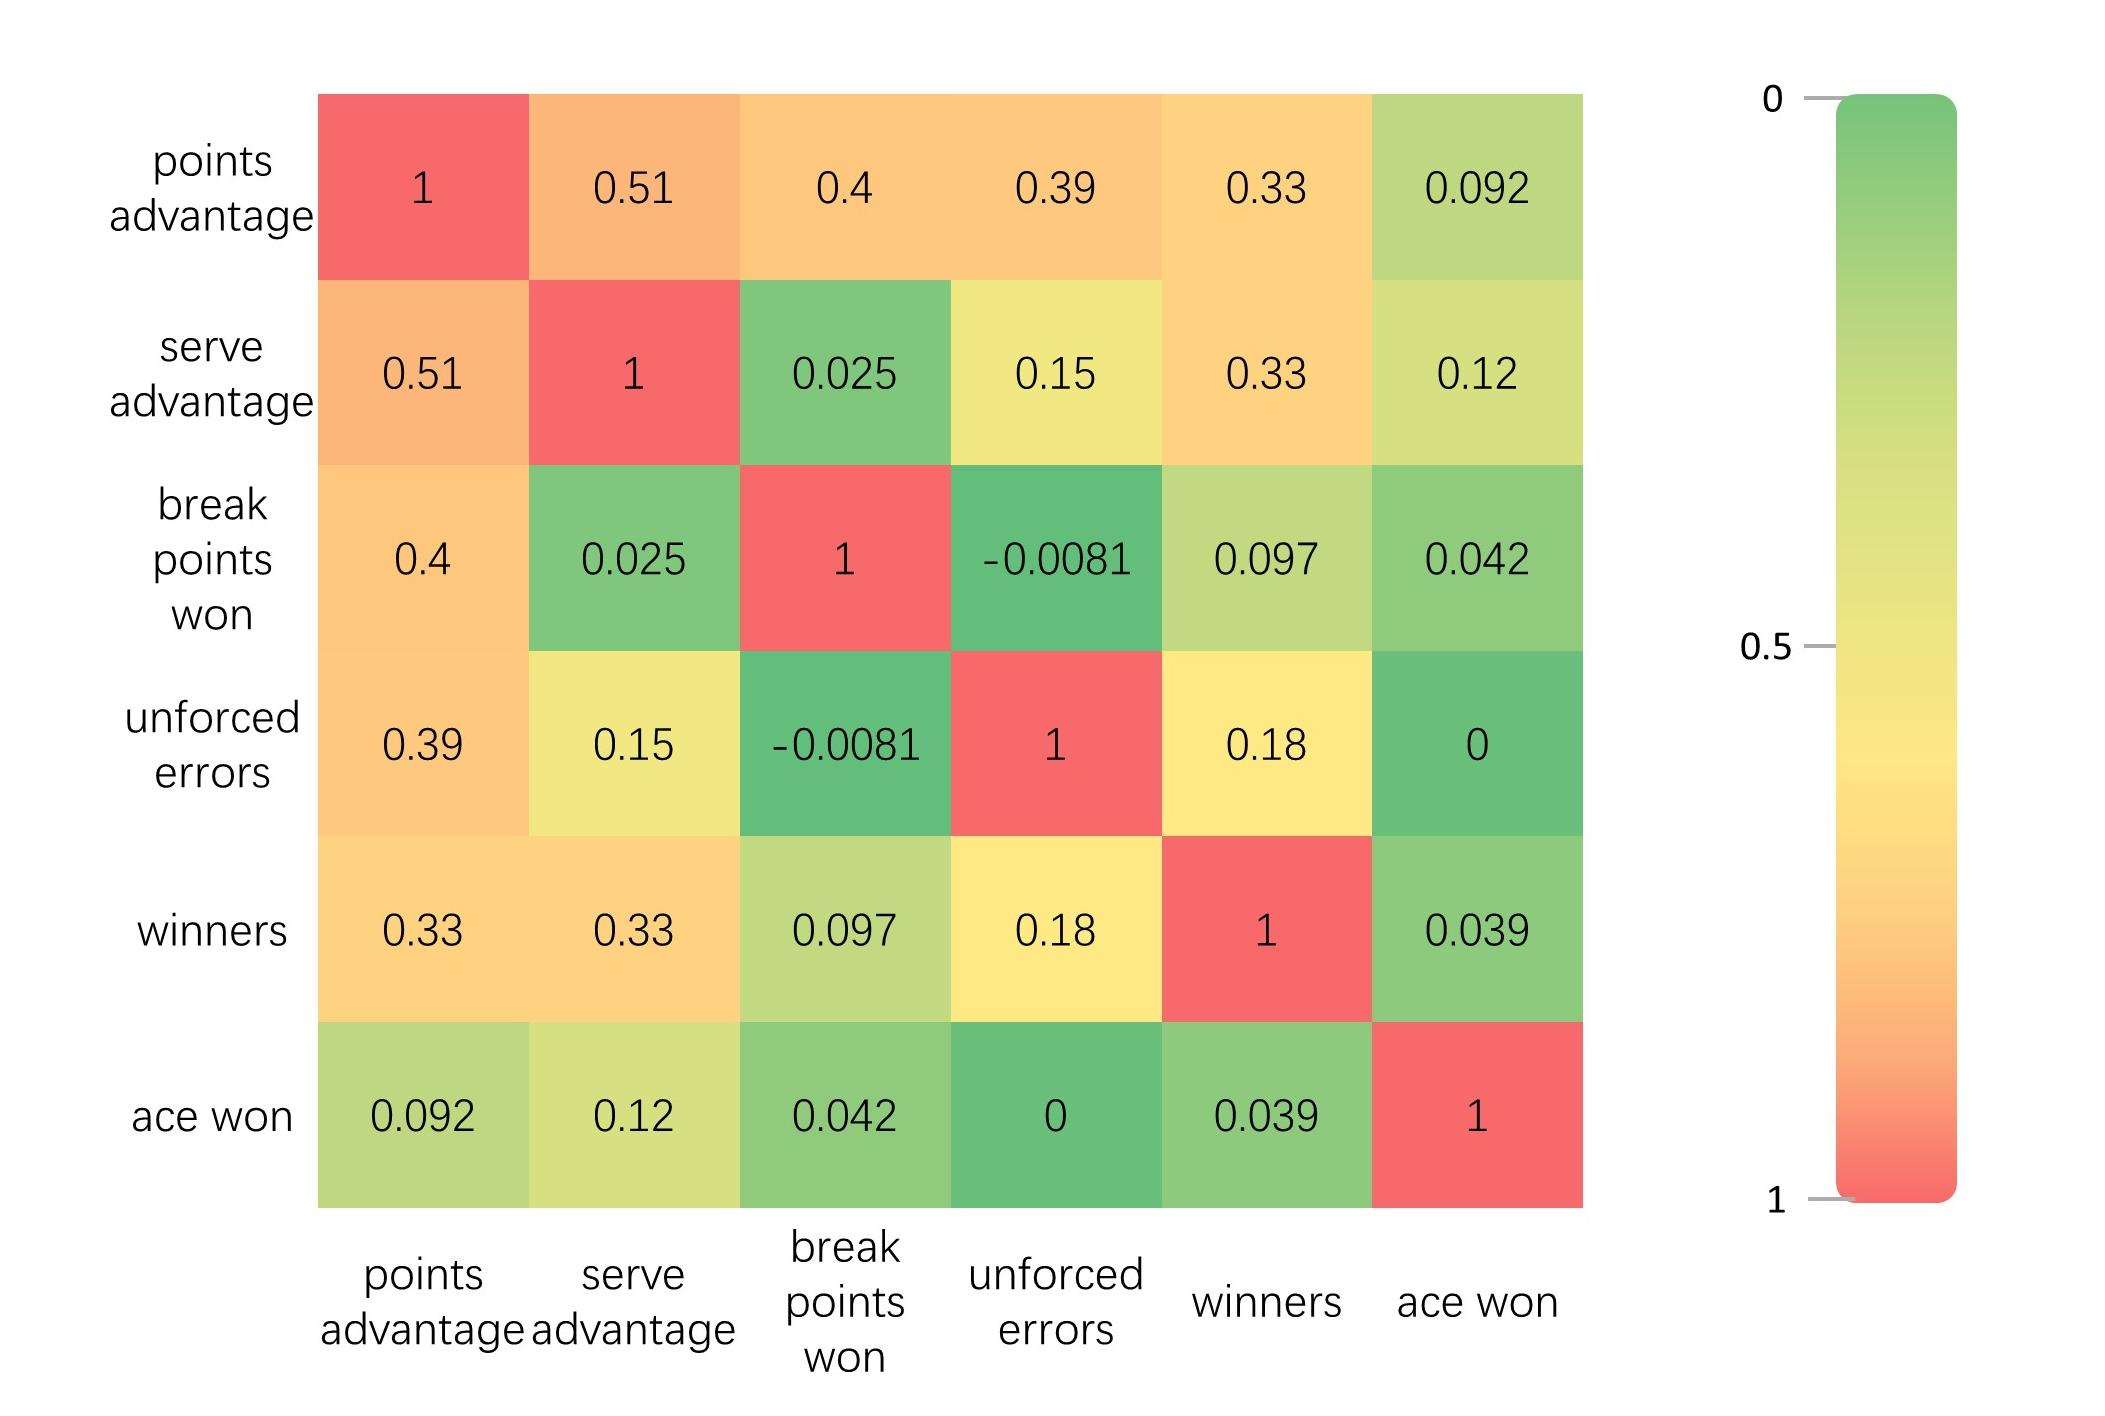
\includegraphics[width=9cm]{figure//hot1.jpg}}% 子图1的相对位置
	\subfigure[For player 2]{				% 图片2
		\label{hot2}						% 子图2的标签
		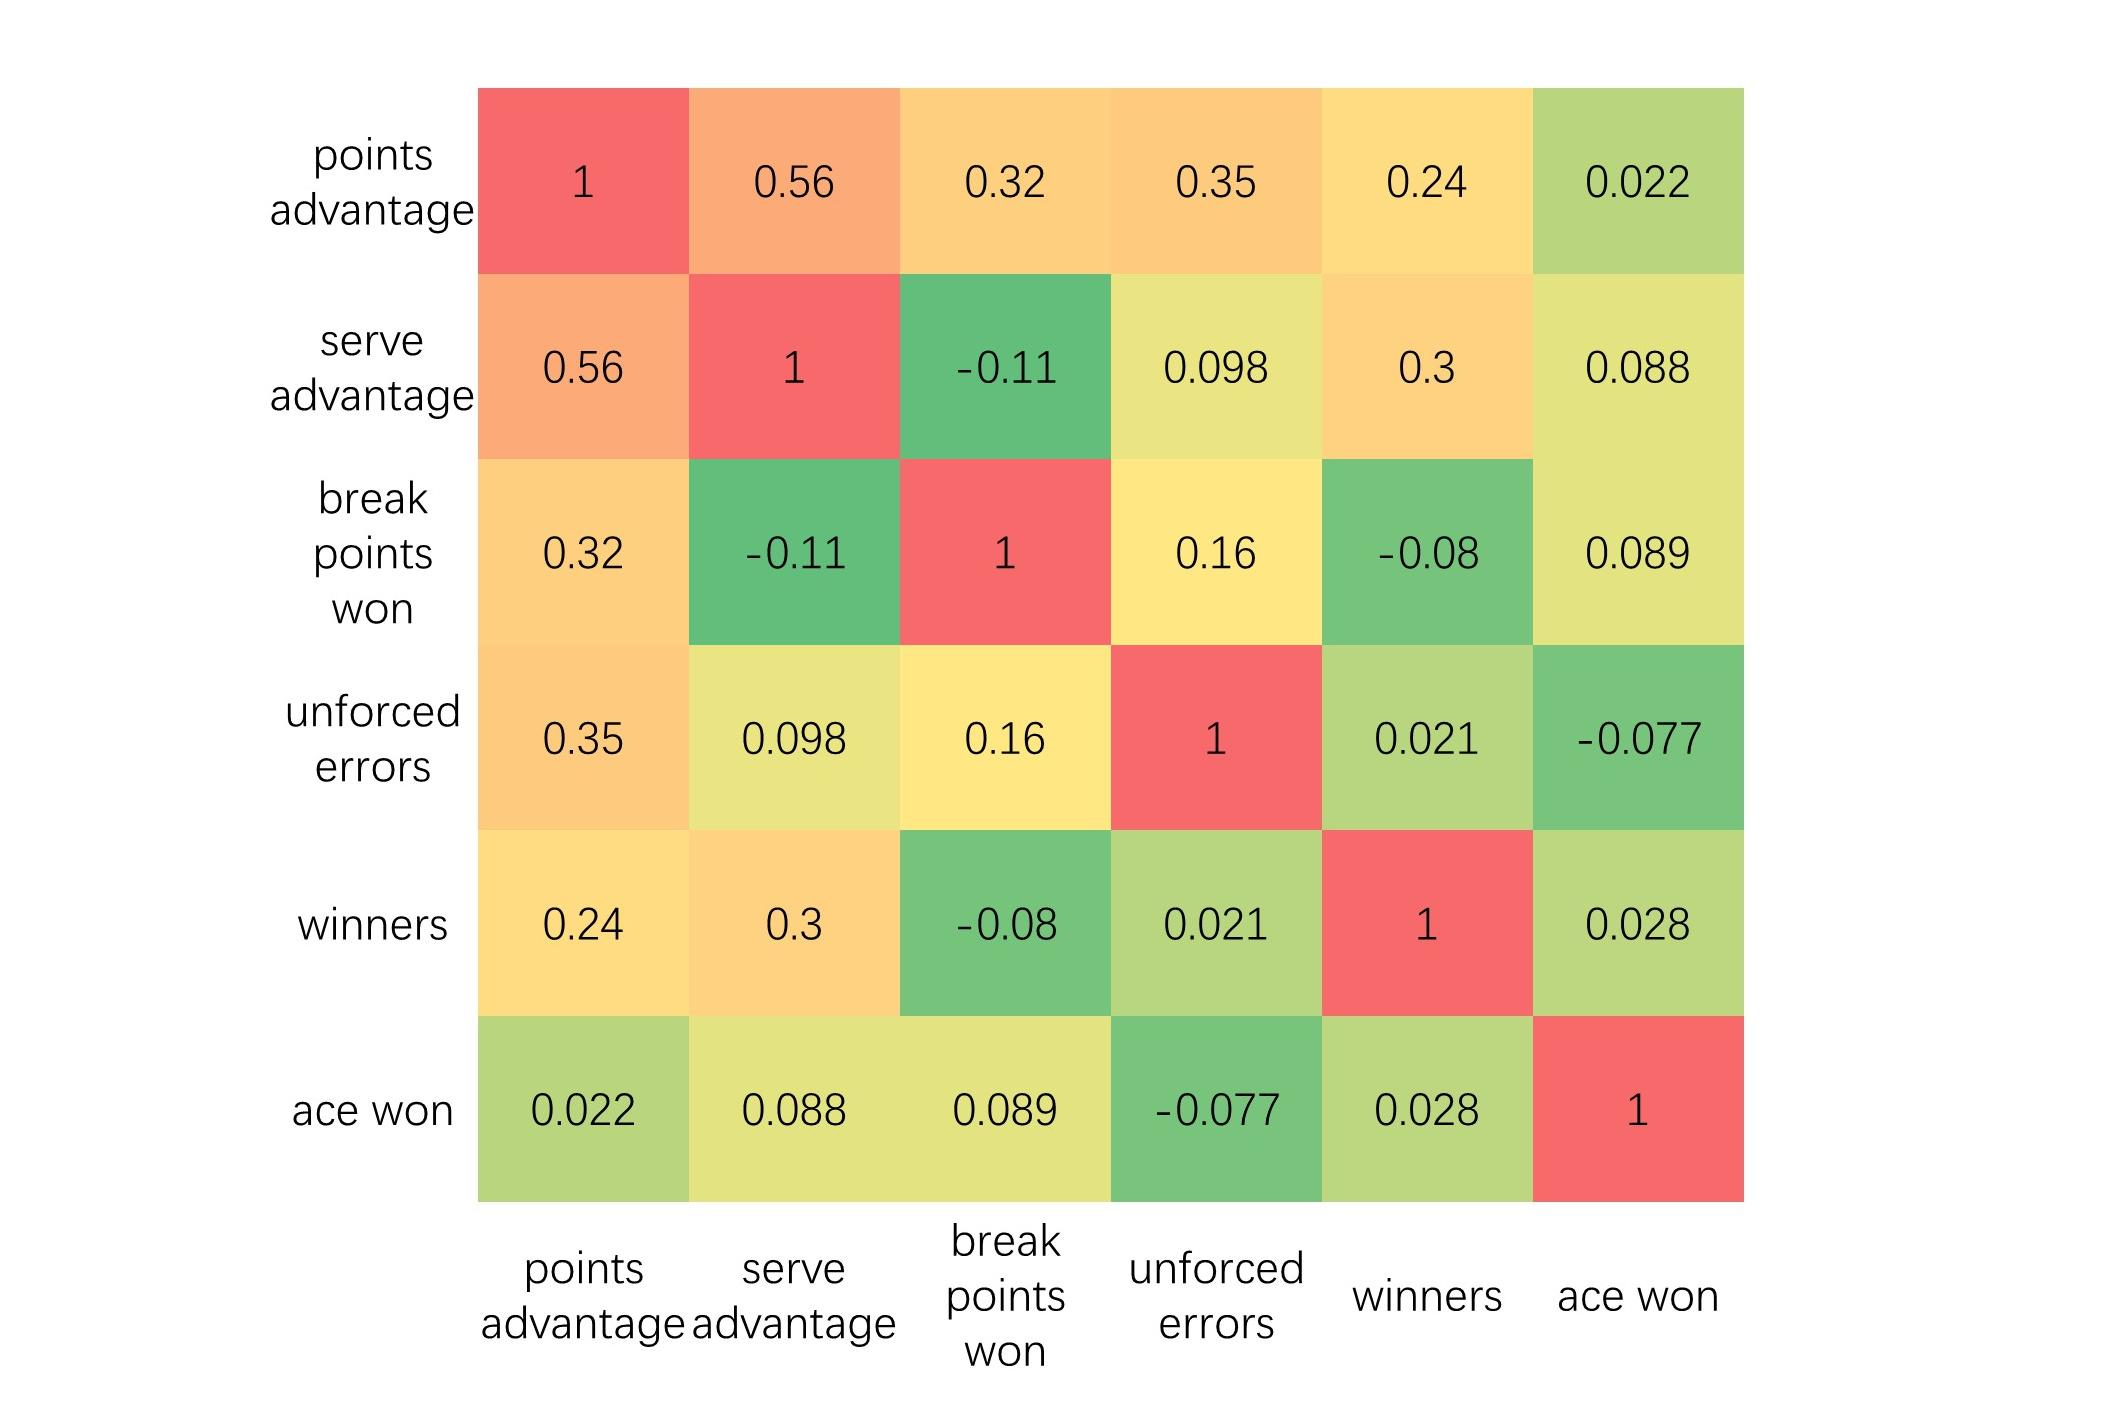
\includegraphics[width=9cm]{figure//hot2.jpg}}% 子图2的相对位置
	\caption{Analysis of the Correlation of Seed Indicators}		% 总图标题
	\label{hot}									% 总图标签
\end{figure}

Figure \ref{hot} reveals the correlations between different match indicators, thereby providing deep insights into player performance. The figure analyses are as following:

1. Point advantage exhibits a positive correlation with winners and serve advantage, which indicates that point advantage is often associated with the improvement of winners and serve advantage. This is logical, as powerful serves and winning shots can directly lead to an increase in points.

2. Break points won has a relatively low correlation with other indicators, which may be because breaking serve is related to specific situations in a match, and these situations may not occur frequently or have a strong direct connection with other indicators.

3. Unforced errors show a negative correlation with most indicators, particularly with point advantage, meaning that an increase in unforced errors may lead to a decrease in point advantage. This also emphasizes the importance of controlling errors to maintain performance in a match.
	
\subsection{Calculate Indicator Entropy} 

We first use to convert negative indicators (Unforced Error) into positive indicators, ensuring the consistency of the data. Then, based on the normalized data, we calculated the information entropy value $E$ for each indicator, using the following formula:
\begin{equation}
E_j=-\frac{1}{\ln (m)} \sum_{i=1}^m p_{i j} \ln \left(p_{i j}\right)
\end{equation}
where \( m \) is the number of samples, and \( p \) is the proportion of the value of the \( i \)-th sample on the \( j \)-th indicator to the sum of all samples for that indicator.\\

Then we use the information entropy values of the indicators to calculate the information entropy redundancy \( d \) for each indicator:

\begin{equation}
	d_j=1-E_j \quad, \quad j=1, 2, 3, \cdots m
\end{equation}
	
Based on the information entropy redundancy \( d \), we calculated the differentiation weight \( W \) for each indicator. The greater the differentiation weight, the more important the role of the indicator in the overall evaluation system. The formula is as follows:

\begin{equation}
	w_j=\frac{d_j}{\sum_{j=1}^m d_j}, j=1, \cdots, m
\end{equation}

Based on the above formulas, we substitute the values of the five indicators and calculate the information entropy value \( e \), the information entropy redundancy \( d \), and the weight \( W \) each indicator holds, as shown in Table \ref{sq1} and Table \ref{sq2}.

\begin{center}
\begin{minipage}{0.9\textwidth}
	\begin{minipage}[t]{0.52\textwidth}
		\begin{table}[H]
			\centering
			\fontsize{9}{11}\selectfont
			\caption{Alcaraz's indicators weight\label{sq1}}
			\begin{tabular}{cccc}
				\toprule[1.5pt]
				\rowcolor{yellow!50}
				Seed Indicators            & E                    & d                    & W                    \\
				\midrule[1pt]
				\rowcolor{yellow!30}
				\cellcolor{orange!40}	points advantage                & 0.989                & 0.010                & 0.018                \\
				\rowcolor{yellow!30}
				\cellcolor{orange!40}serve advantage
				& 0.938                & 0.061                & 0.104              \\
				\rowcolor{yellow!30}
				\cellcolor{orange!40}break points won
				& 0.612                & 0.388                & 0.656               \\
				\rowcolor{yellow!30}
				\cellcolor{orange!40}unforced errors
				& 0.976                & 0.023                & 0.040              \\
				\rowcolor{yellow!30}
				\cellcolor{orange!40}winners
				& 0.934                & 0.066                & 0.111               \\
				\rowcolor{yellow!30}
				\cellcolor{orange!40}ace won
				& 0.993                & 0.006                & 0.010              \\
				\bottomrule[1.5pt]
				\multicolumn{1}{l}{} & \multicolumn{1}{l}{} & \multicolumn{1}{l}{} & \multicolumn{1}{l}{} \\
				\multicolumn{1}{l}{} & \multicolumn{1}{l}{} & \multicolumn{1}{l}{} & \multicolumn{1}{l}{}
				\label{w}
			\end{tabular}
			\vspace{3pt}
		\end{table}
	\end{minipage}
	% 中间不能有空格,否则不会并排显示
	\begin{minipage}[t]{0.52\textwidth}
		\begin{table}[H]
			\centering
			\fontsize{9}{11}\selectfont
			\caption{Djokovic's indicators weight\label{sq2}}
			\begin{tabular}{cccc}
				\toprule[1.5pt]
				\rowcolor{yellow!50}
				Seed Indicators            & E                    & d                    & W                    \\
				\midrule[1pt]
				\rowcolor{yellow!30}
				\cellcolor{orange!40}	points advantage                
				& 0.977                & 0.023                & 0.037                \\
				\rowcolor{yellow!30}
				\cellcolor{orange!40}serve advantage
				& 0.960                & 0.040                & 0.066              \\
				\rowcolor{yellow!30}
				\cellcolor{orange!40}break points won
				& 0.612                & 0.388                & 0.633               \\
				\rowcolor{yellow!30}
				\cellcolor{orange!40}unforced errors
				& 0.992                & 0.008                & 0.014              \\
				\rowcolor{yellow!30}
				\cellcolor{orange!40}winners
				& 0.884                & 0.116                & 0.189               \\
				\rowcolor{yellow!30}
				\cellcolor{orange!40}ace won
				& 0.999                & 0.001                & 0.002              \\
				\bottomrule[1.5pt]
				\multicolumn{1}{l}{} & \multicolumn{1}{l}{} & \multicolumn{1}{l}{} & \multicolumn{1}{l}{} \\
				\multicolumn{1}{l}{} & \multicolumn{1}{l}{} & \multicolumn{1}{l}{} & \multicolumn{1}{l}{}
				\label{w}
			\end{tabular}
			\vspace{3pt}
		\end{table}
	\end{minipage}
\end{minipage}
\end{center}


From Table \ref{sq1}, it can be seen that Alcaraz's indicators are focused on the number of break points won, winners, and serve advantage, which reflects that the number of break points won, the number of winners hit, and whether being the server have the greatest impact on the player's overall performance in matches.

From Table \ref{sq2}, we find that Djokovic's indicators also show that the number of break points won and the winners have a significant impact on his performance. Compared to Alcaraz, winners have a slightly greater impact on Djokovic, which suggests that Djokovic adopts a more aggressive offensive strategy during matches.

\subsection{Calculate the Performance Score} 
	
Based on the weights of each indicator determined by the entropy weight method, the formula for calculating the final performance score \( B \) is as follows: 

\begin{equation}
	B=W_{1}x_1+W_{2}x_2+W_{3}x_3+W_{4}x_4+W_{5}x_5+W_{6}x_6
\end{equation}

where \( W \) is the weight of each indicator, \( x \) is the actual score of each indicator.
	
%%%%%引入获胜概率????

\subsection{Results Visualization}
\subsubsection{Time Series Chart}

The Figure \ref{r3} shows the changes in the composite performance scores of player 1 and player 2 during the finals. By comparing the score changes of the two players, we can observe the trends of their performance fluctuations in different matches.
\begin{figure}[H]
	\centering
	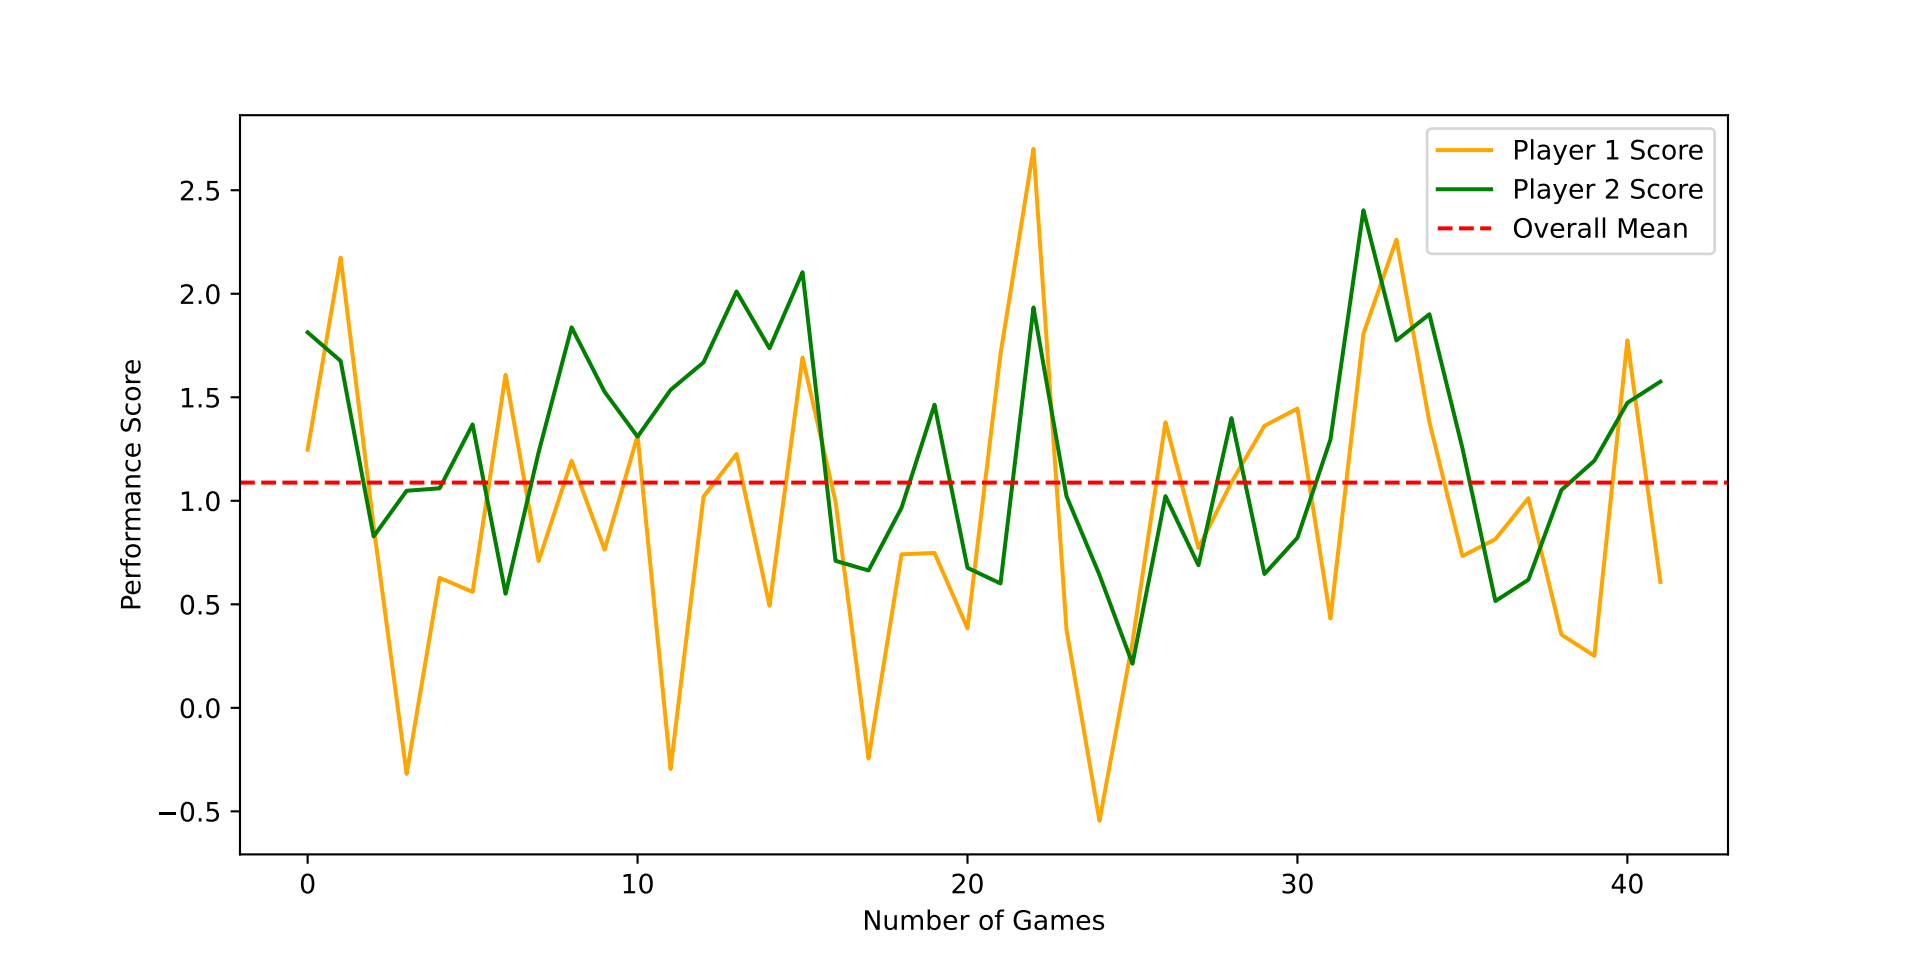
\includegraphics[scale=0.5]{figure//p1r.png}
	\caption{Explained Variance Cumulation by PCA Components}
	\label{p1r}
\end{figure}

From the Figure \ref{p1r}, we can observe some conclusions as following:

 Player 1's composite performance score shows certain fluctuations, indicating instability in their match performance. The variability of their scores may be related to the strength of the opponents, changes in match strategy, or fluctuations in the player's own condition.

Player 2's composite performance score also exhibits fluctuations. However, in some games, player 2's score is significantly higher than1, suggesting that player 2 may have demonstrated stronger overall abilities or implemented effective match strategies in these games.

By comparing the performance scores of the two players, coaches and players can better understand their own strengths and weaknesses, thereby making targeted training and strategic adjustments to improve match performance.



\subsubsection{Match Charging Chart}

In order to more interestingly reflect the impact of the performance scores we proposed on match outcomes, we create a player battery indicator chart.

Based on the average performance score of the players throughout the match, we divide their performance scores into four levels, represented by four battery levels: full battery indicates an excellent performance score by the player. As the battery level decreases, the player's performance score becomes progressively lower; the letter "W" in a tennis represents winning the game, and the letter "L" represents losing the game.


\begin{figure}[H]
	\centering
	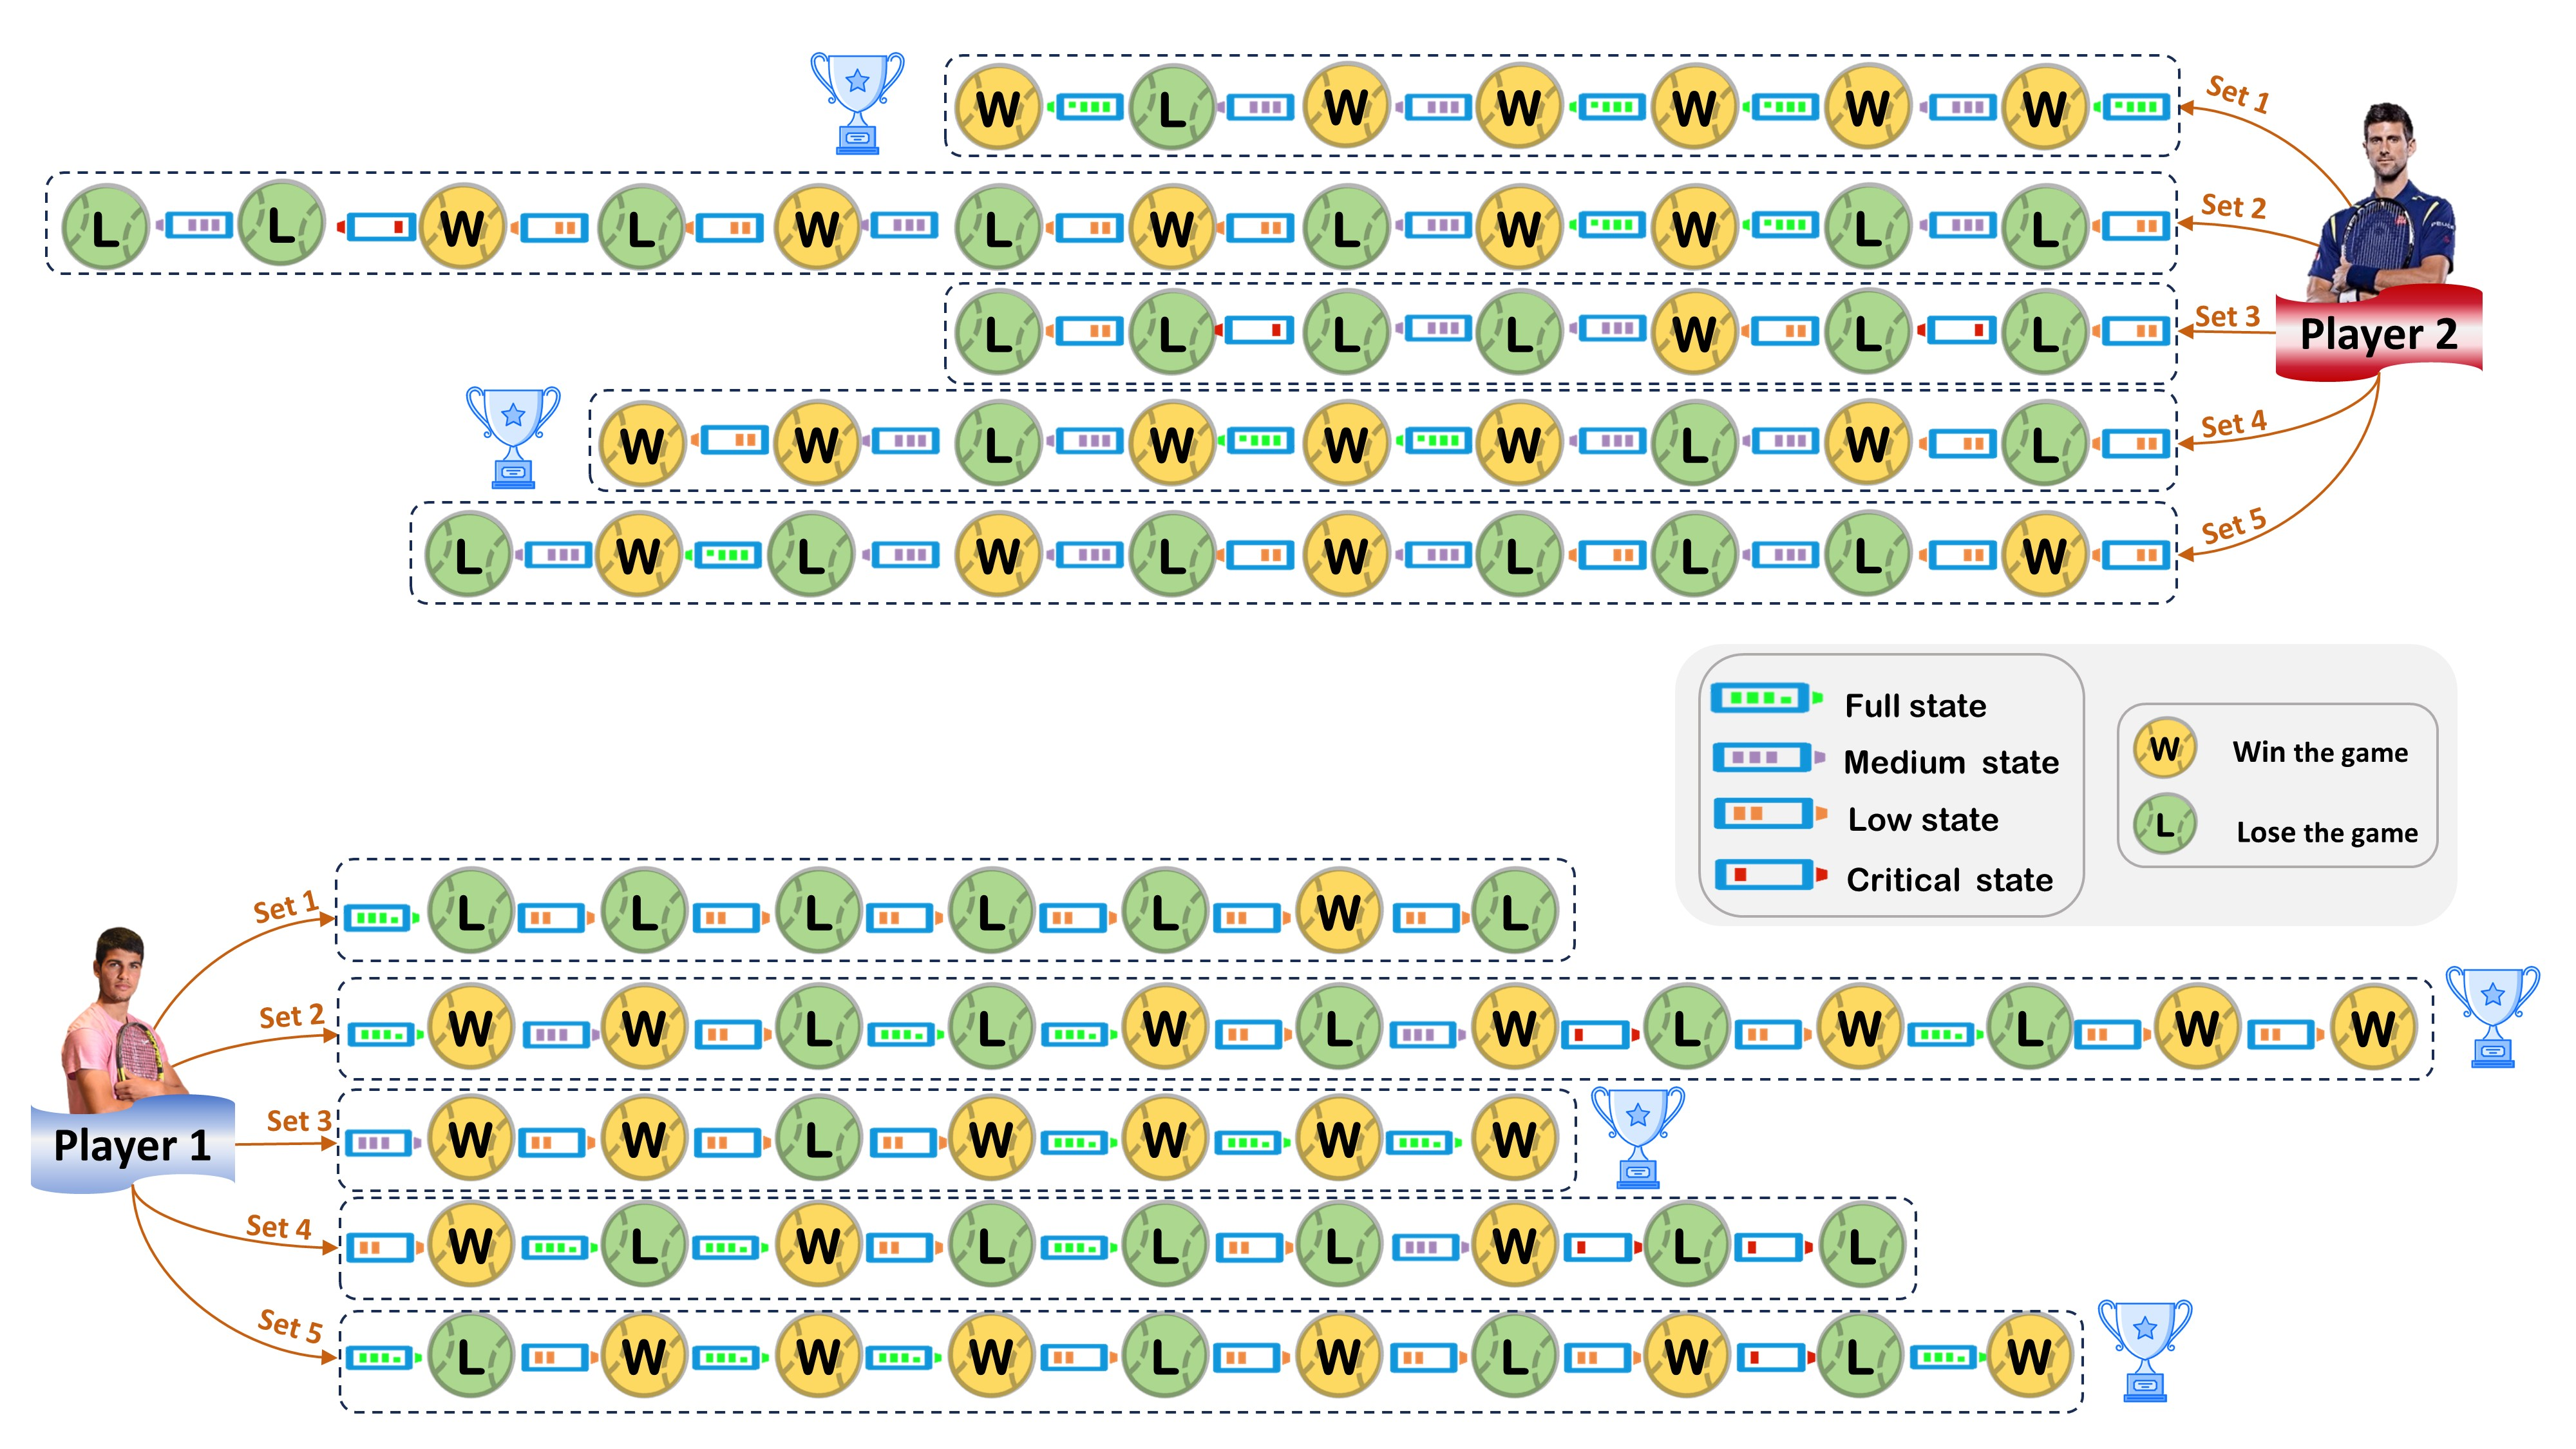
\includegraphics[scale=0.5]{figure//1r3.jpg}
	\caption{Djokovic and Alcaraz's match charging chart}
	\label{r3}
\end{figure}

The figure shows that the performance score we proposed is highly correlated with the outcome of each game. When the battery is fully charged, that is, when the performance score for the set is high, players tend to win the game; conversely, when the battery is low, the probability of a player losing is significantly high.

 Interestingly, we found that the young Alcaraz always starts each set with a lot of energy and a high performance score. However, as the match progresses, their performance fluctuates significantly with the wins and losses. This may indicate that their ability to adjust and cope under pressure and adverse situations needs to be strengthened. In contrast, the experienced Djokovic, despite starting slowly at the beginning of each set, can effectively control the impact of the match's progress on their state, displaying strong mental resilience and strategic adjustment capabilities, thereby making the performance more stable as the game unfolds.






\section{Tennis Momentum Volatility via Run Test}
\subsection{Definition of Momentum}
\begin{itemize}
	\setlength{\parsep}{0ex} %段落间距
	\setlength{\topsep}{2ex} %列表到上下文的垂直距离
	\setlength{\itemsep}{1ex} %条目间距
	\item \textbf{Explanation of Momentum:} ``Momentum" typically refers to a player's trend of consecutive wins or scoring in a match, which can persist for some time before potentially abruptly changing. It emphasizes the streak of victories or consistent scoring within a game \cite{gao2021random}, usually focusing on the overall dynamics of the match.
	
	\item \textbf{Explanation of Performance:} ``Performance" generally signifies one side’s outstanding execution in a particular set or over a period, often in relation to positive factors such as scoring, serving, receiving, etc. Quantifying "performance" can be based on various match statistics, highlighting the specific technical and strategic performance within a set or period, with an emphasis on the short-term situation of the match.
	
	\item \textbf{ Definition of ``Momentum":}  In tennis matches, momentum is often a combination of ``performance" and physical condition. Given the difficulty in estimating the physical condition of players, we overlook each player's physical state and its impact on their game, which we have made the justification in Assumption. Therefore, we approximate momentum with ``performance points." The indicators that affect ``performance points" are equally applicable to ``momentum."
\end{itemize}
\subsection{Randomness Test Based on Run Test}
To verify the randomness of players' winning streaks and turning points in matches, we propose a method using the run test, which examines momentum and turning points to determine if the sample is random. The formula is as following: 
\begin{equation}
	Z_x=W(x)=\frac{(2n_1*n_2+n)}{n} \\
\end{equation}
\begin{equation}
\sigma^2_x=\frac{2n_1n_2(2n_1n_2-n)}{n^2(n-1)}
\end{equation}

Then, we can derive the statistic:
\begin{equation}
	R=\frac{-Z_x+r}{\sigma}\sim N(0,1)
\end{equation}
where \( r \) represents the total number of runs, \( n_1 \), and \( n_2 \) respectively signify the number of times the price increased and decreased. \( n \) is the total sample size, i.e., \( n_1 + n_2 = n \). Thus, when \( n \) is large, \( x \) approximately follows a normal distribution. Assuming \( Z_x \) is the expected value under normal distribution and \( \sigma \) is the variance.

\begin{table}[htbp]
	\centering
	\caption{Run Test Results}
			\label{22222}
	\begin{tabular}{lccc}
		\toprule
		\rowcolor{orange!40}
		Name & Sample Size & z & P \\
		\midrule
		p1\_momentum & 334 & -11.9431 & 0.000*** \\
		p2\_momentum & 334 & -12.0528 & 0.000*** \\
		\bottomrule

	\end{tabular}
	
	\smallskip
	\textit{Note: ***,**,* represent significance levels of 1\%, 5\%, 10\%, respectively.}
\end{table}



\subsection{ Multiple Match Testing}
By conducting run tests on all matches and summarizing the results as shown in the following table.

\begin{table}[h] \centering \caption{Partial Match Inspection Data}
	\resizebox{\textwidth}{!}{ \begin{tabular}{cccccc} \toprule 
					\rowcolor{orange!40} Row & Match ID & p1\_momentumisRand & p2\_momentumisRand & p1\_turning\_pointsisRand & p2\_turning\_pointsisRand \\ \midrule 0 & 2023-wimbledon-1301 & 1 & 1 & 0 & 0 \\ 1 & 2023-wimbledon-1302 & 1 & 1 & 0 & 0 \\ 2 & 2023-wimbledon-1303 & 1 & 1 & 0 & 0 \\ 3 & 2023-wimbledon-1304 & 1 & 1 & 0 & 1 \\ 4 & 2023-wimbledon-1305 & 1 & 1 & 0 & 1 \\ \addlinespace \multicolumn{6}{c}{\dots} \\ \addlinespace 26 & 2023-wimbledon-1503 & 1 & 1 & 1 & 0 \\ 27 & 2023-wimbledon-1504 & 1 & 1 & 1 & 0 \\ 28 & 2023-wimbledon-1601 & 1 & 1 & 0 & 0 \\ 29 & 2023-wimbledon-1602 & 1 & 1 & 1 & 0 \\ 30 & 2023-wimbledon-1701 & 1 & 1 & 1 & 1 \\ \bottomrule \end{tabular} }\end{table}

Reviewing the momentum changes for p1 and p2, it is clear that all matches exhibit non-randomness in terms of players' momentum. All values are 1, which may be due to various factors such as the actual level of the players, tactics, etc.


\section{GSRF Model for Tennis Momentum Prediction}
In this section, we aim to explore the momentum fluctuations in tennis matches, especially when the flow of the match may shift from favoring one player to another. By analyzing momentum fluctuations in multiple past matches, we employ a GSRF (Grid Search-based Random Forest Regression) model to predict the fluctuation differences in upcoming games, thus analyzing the reasons for the internal fluctuations.
\subsection{Definition of Match Fluctuation}
We analyze the fluctuation situation in a match by taking the difference in momentum between the two players as the match fluctuation.


\subsection{Match Fluctuation Prediction Based on GSRF}

Based on the results of correlation and PCA analysis, we selected the six indicators with the highest correlation coefficients as shown in Table \ref{222}.
\begin{table}[H]
	\centering
	\caption{Top 8 principal variables}
	\begin{tabular}{cccc}
		
		\hline
		\hline
		\rowcolor{orange!50}
		Indicators          & PC1      & PC2       &                      \\
		\hline
		\cellcolor{yellow!30}
		p1\_ace            & 0.737698 & 0.68423   &                      \\
		\cellcolor{yellow!30}
		p1\_break\_pt\_won & 0.046219 & 0.030478  &                      \\
		\cellcolor{yellow!30}
		p1\_winner         & 0.811273 & 0.088375  &                      \\
		\cellcolor{yellow!30}
		p1\_unf\_err       & 0.24327  & 0.374712  &                      \\
		\cellcolor{yellow!30}
		p1\_net\_pt\_won   & 0.346378 & 0.665525  &                      \\
		\cellcolor{yellow!30}
		server             & 0.569129 & 0.605448  & \multicolumn{1}{l}{} \\
 \hline \hline
		&          &           & \multicolumn{1}{l}{}
		\label{222}
	\end{tabular}
\end{table}




 Using these indicators, we adopted a GSRF (Grid Search-based Random Forest Regression model) to predict momentum fluctuations in matches. By generating10,000 resampled datasets via bootstrapping, we trained the random forest to accurately predict fluctuations during matches.
 
 In addition, we also compared the effects of two hyperparameter optimization strategies, grid search and genetic algorithms, on model performance. The specific random forest process is shown in the following Figure \ref{sl}.

\begin{figure}[H]
	\centering
	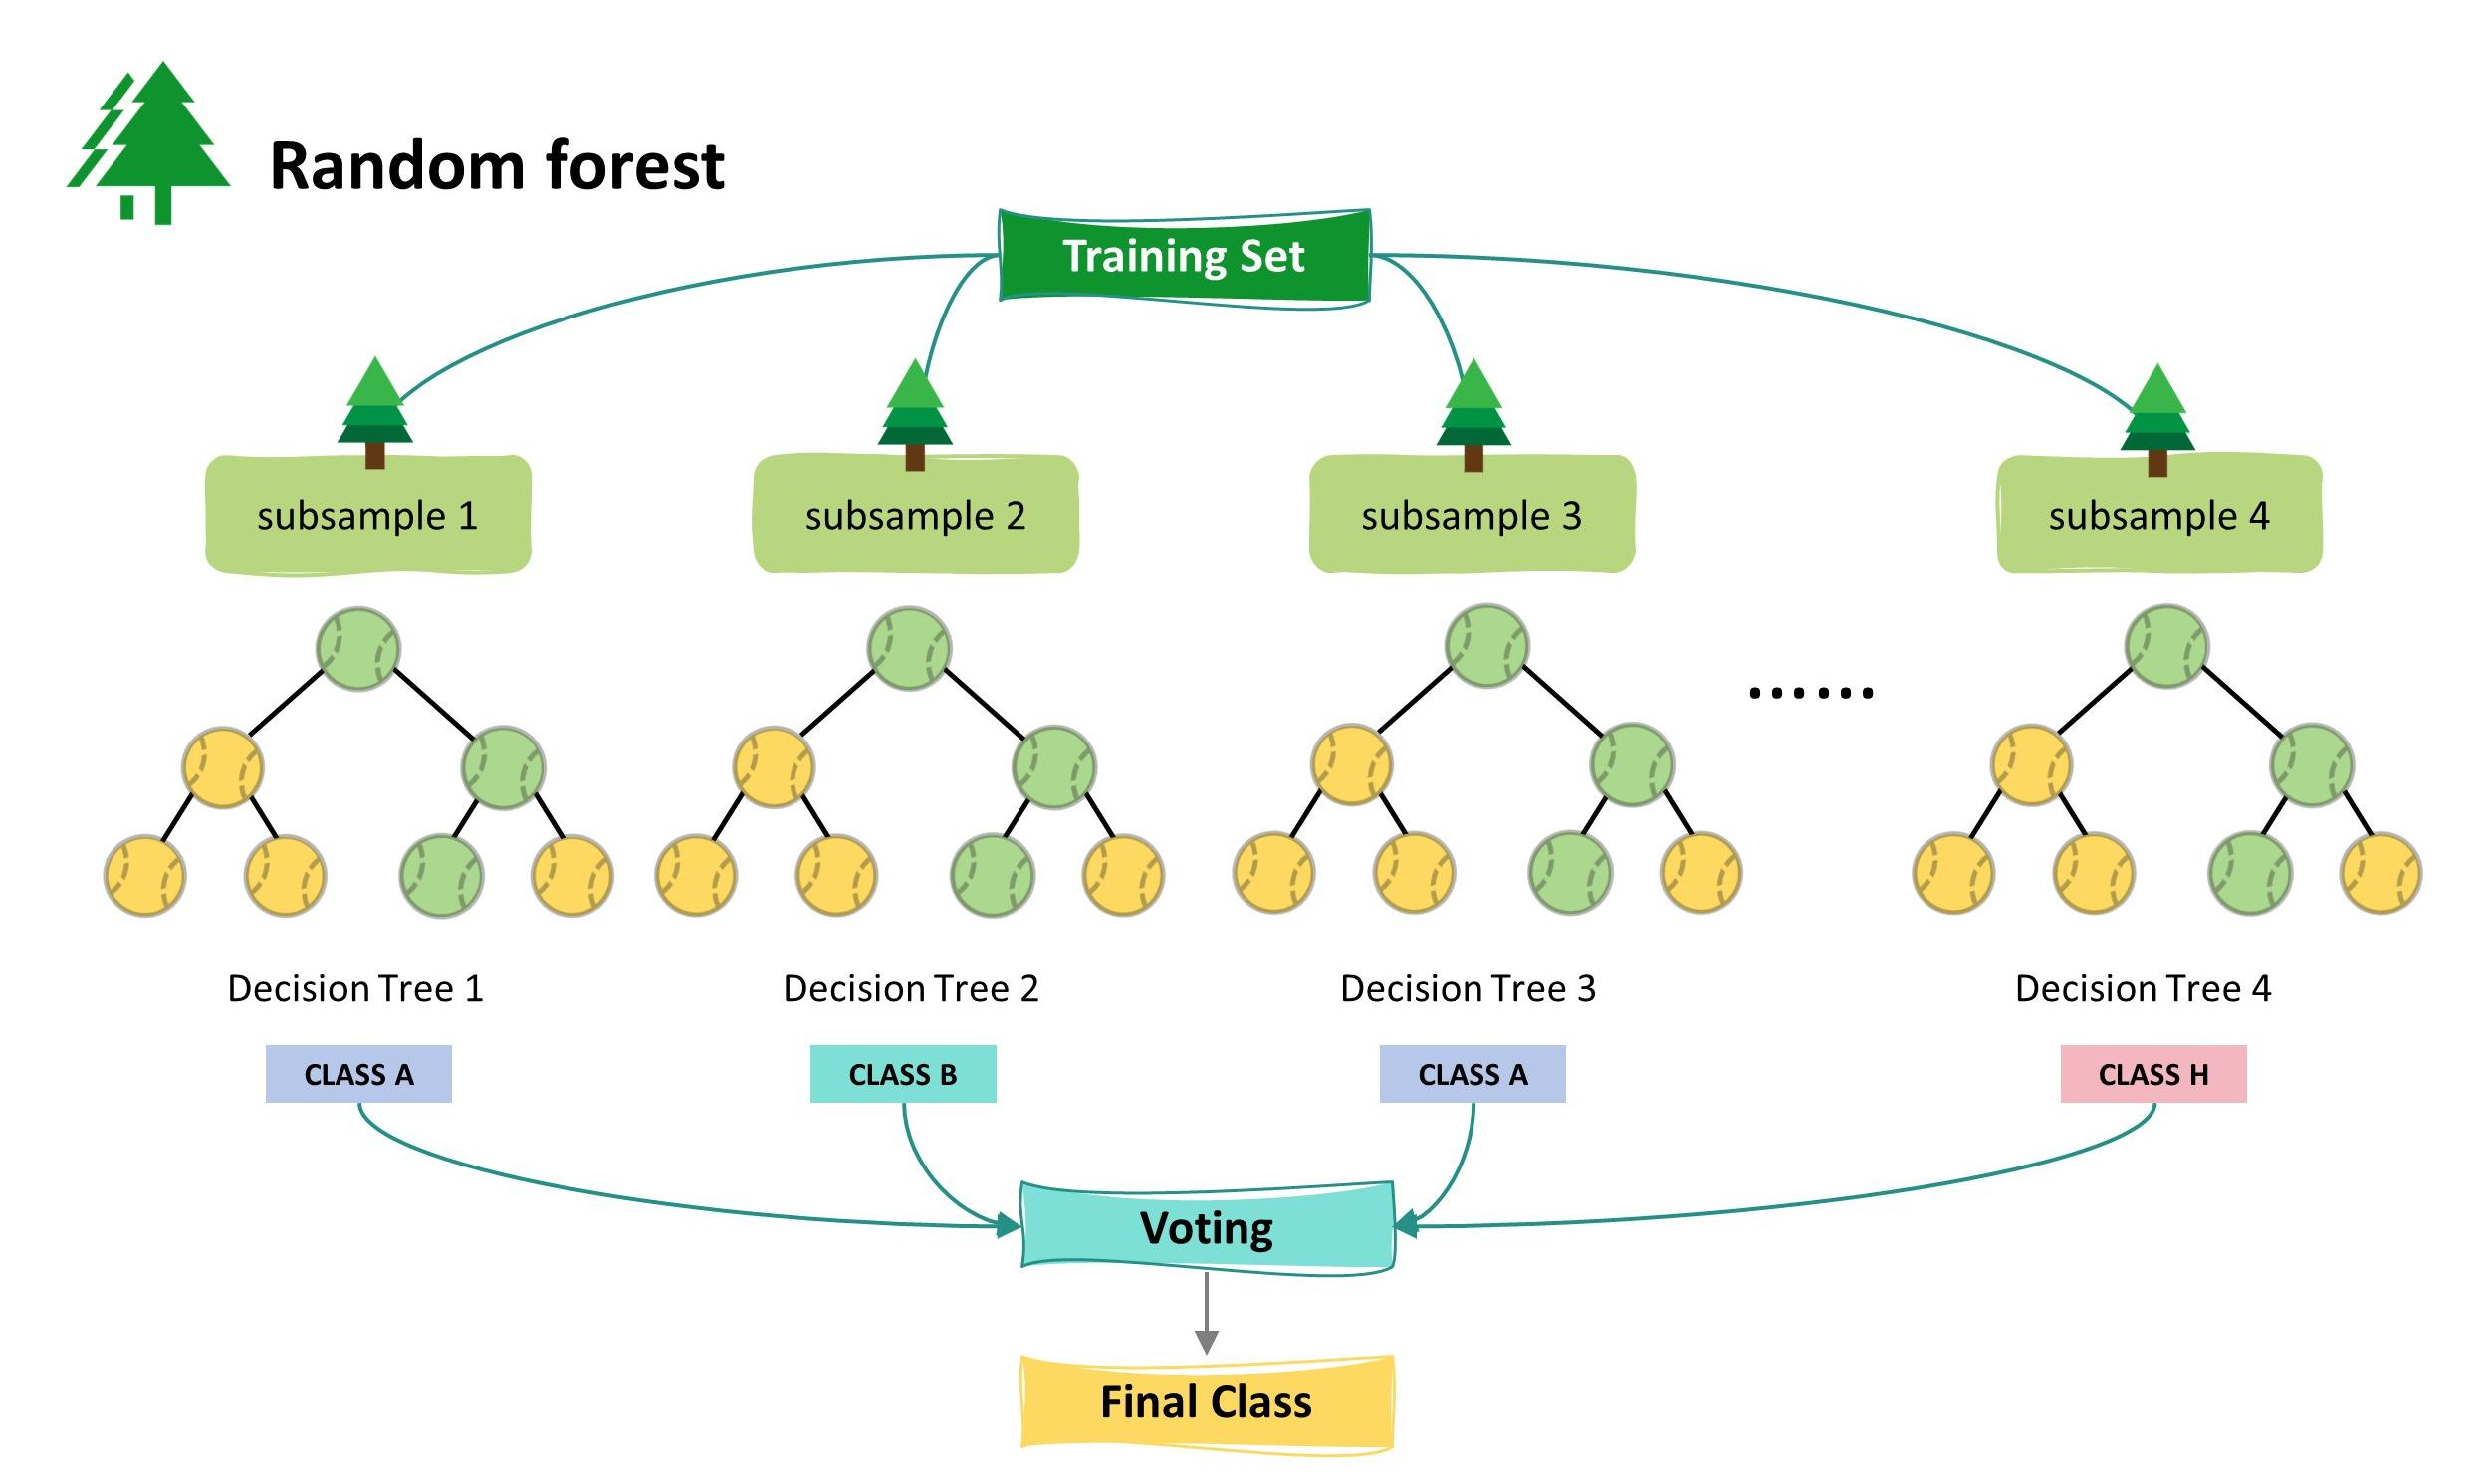
\includegraphics[scale=0.42]{figure//sl.jpg}
	\caption{Random forest}
	\label{sl}
\end{figure}

\subsection{Model Evaluation and Selection}

We further implemented two different hyperparameter optimization strategies to evaluate the impact of hyperparameter optimization on the performance of the random forest model: Grid Search and Genetic Algorithm. Grid Search determines the best hyperparameter configuration by systematically traversing all possible combinations of parameters. In contrast, the Genetic Algorithm searches for the optimal set of hyperparameters by simulating the genetic mechanisms in the process of natural selection, navigating through the hyperparameter space with crossover, mutation, and selection operations, aiming to find a set of hyperparameters that enhance model performance. \\

In order to comprehensively evaluate and compare the performance of the two predictive models, we use MAPE (Mean Absolute Percentage Error) and the $R^2$ (Coefficient of Determination) to measure the performance of the two models. \\

MAPE is a metric used to measure the percentage error between predicted values and actual values. Its formula is as follows:
\begin{equation}
MAPE = \frac{1}{n} \sum_{i=1}^{n} \left| \frac{Y_i - \hat{Y}_i}{Y_i} \right| \times 100
\end{equation}
where
$n$ is the number of observations.
$Y_i$ is the actual observed value.
$\hat{Y}_i$ is the predicted value for the corresponding observation.
A lower MAPE value indicates that the model is more accurate in its predictions, as the percentage error is smaller.\\

$R^2$ measures the degree to which the model explains the variance in the dependent variable, with values ranging between 0 and 1. Its formula is as follows:
\begin{equation}
	R^2 = 1 - \frac{\sum_{i=1}^{n} (Y_i - \hat{Y}_i)^2}{\sum_{i=1}^{n} (Y_i - \bar{Y})^2}
\end{equation}

where $ n $ is the number of observations.
$ Y_i $ is the actual observation value.
$\hat{Y}_i $ is the predicted value for the corresponding observation.
$\bar{Y} $ is the average value of the observations.

R² is used to evaluate the explanatory power of the model for the variations in the target variable. The value of R² ranges from 0 to 1, with a value closer to1 indicating that the model can more fully explain the variations in the target variable. A higher R² indicates that the model fits the data better.

\begin{figure}[H]
	\centering
	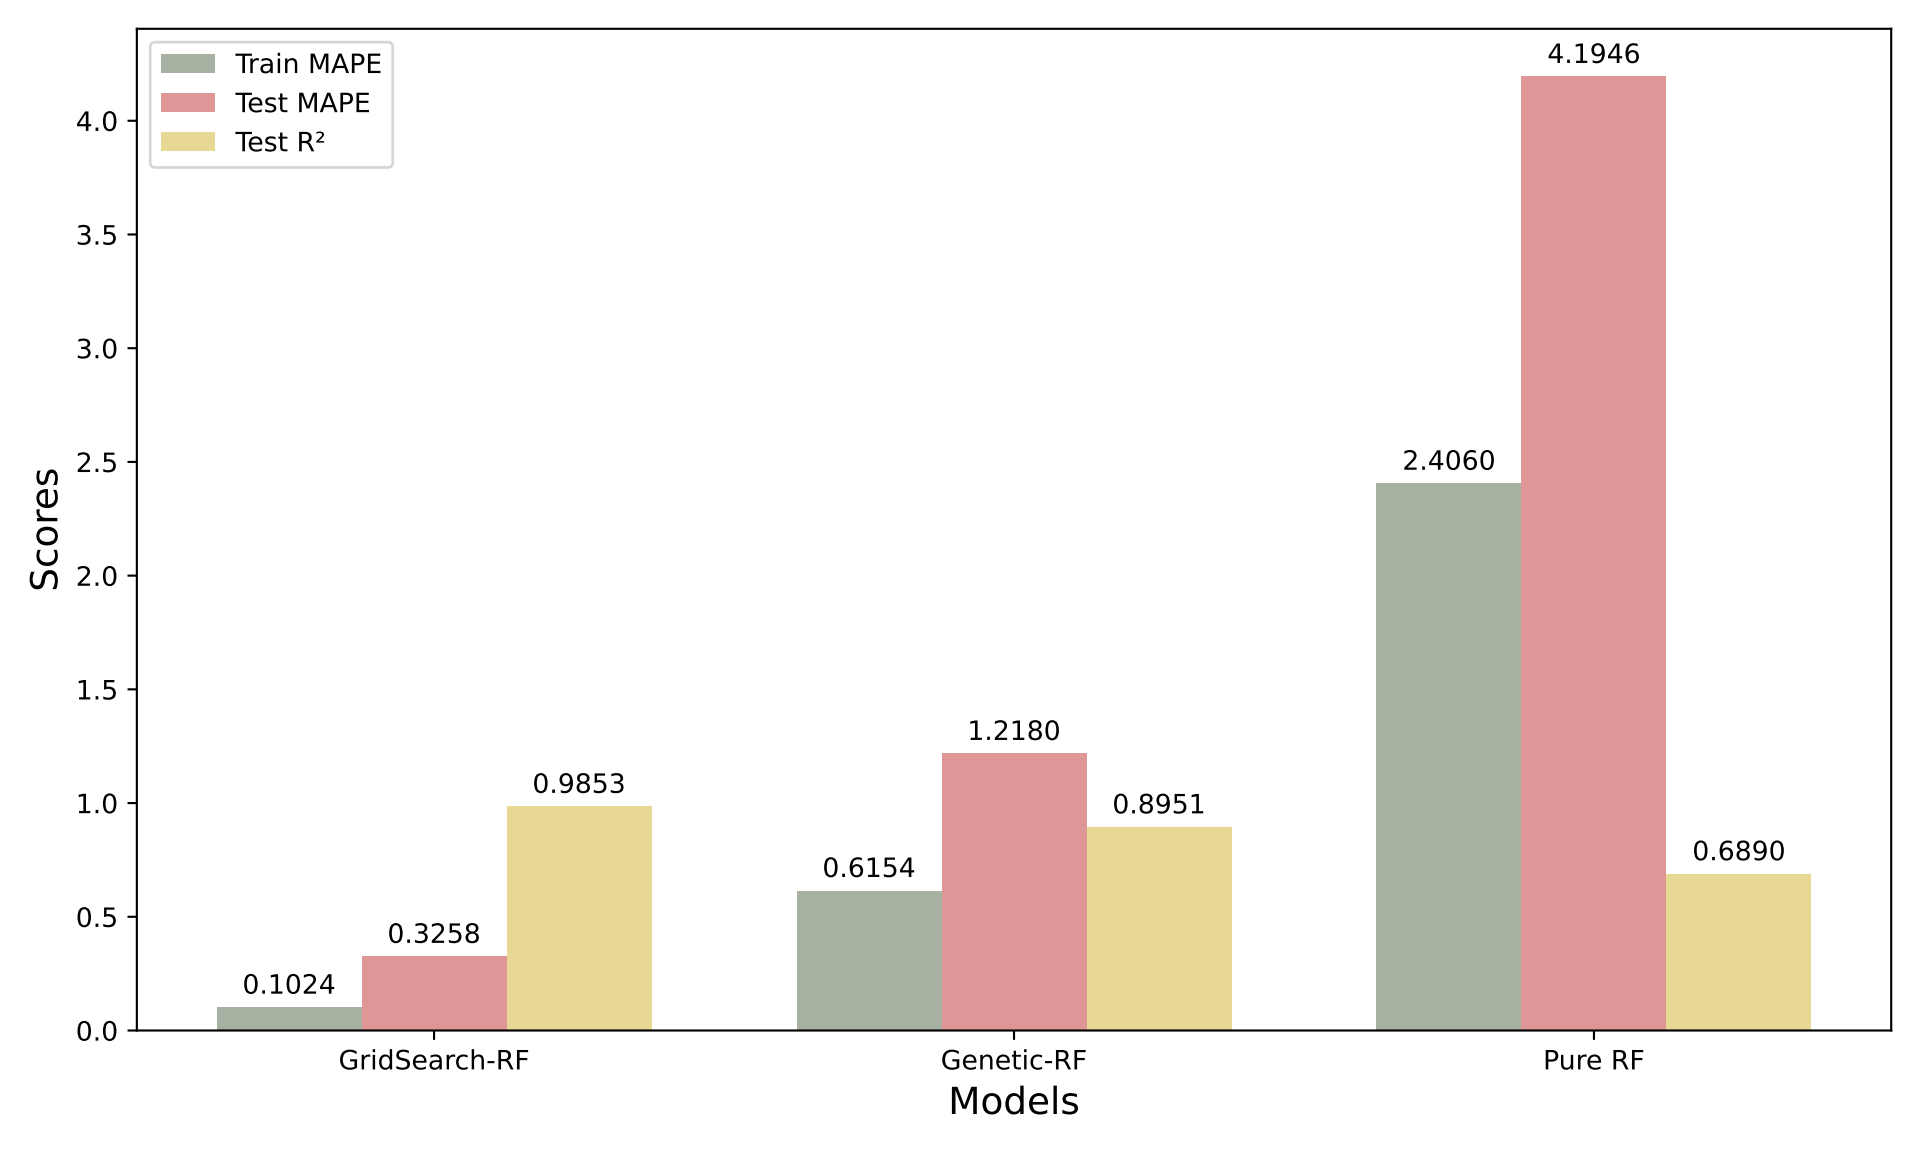
\includegraphics[scale=0.5]{figure//sl2.png}
	\caption{Model performance comparison}
	\label{sl2}
\end{figure}

According to Figure \ref{sl2}, the Test MAPE value for the grid search-based random forest is 0.124, which is significantly lower than the value obtained from the random forest based on the genetic algorithm. This indicates that the former is more accurate in prediction, and the GSRF's $R^2$ (0.9853) is also slightly higher than the $R^2$ (0.8951) based on the genetic algorithm, indicating that the former also has a better degree of fit.


\subsection{Momentum Differences and Turning Points}
Definition of a turning point: A point where continuous scoring shifts to continuous losing of points, or vice versa, represented in the CUMSUM algorithm as points where the cumulative sum equals zero.


\subsection{Calculation of Momentum Difference Sequence}
To better quantify the magnitude of momentum change at each time point, we first perform a differencing operation on the momentum of each player to calculate the potential energy difference between two points. The time series formula is denoted as $G(t)$, where $t=1,2,...,n$. Therefore, the difference sequence $D(t)$ is represented as:
\begin{equation}
 D(t) = G(t) - G(t-1) 
\end{equation}
where D(t) represents the amount of momentum change between time $t$ and $t-1$.

Each value in the difference sequence can effectively reflect the real-time changes in each player's performance; a positive value indicates an increase in momentum, while a negative value indicates a decrease in momentum.

\subsection{The Use of CUMSUM}
The Cumulative Sum (CUMSUM) algorithm identifies shifts in momentum by accumulating positive and negative changes in a differential series. Momentum changes over time are captured by calculating the cumulative total of the differential series. A significant change in the CUMSUM curve indicates a potential turning point. The formula is as following:
\begin{equation}
F(t)=\sum^t_{i=1}D(i)
\end{equation}
where $F(t)$ represents the cumulative change in momentum up to time $t$. CUMSUM can identify potential turning points by observing the trends in $F(t)$.
Based on the CUMSUM results , we extracted turning points from these cumulative sum curves, which indicate shifts in momentum trends \cite{KNOTTENBELT20123820} during the match.
\begin{figure}[H]
	\centering
	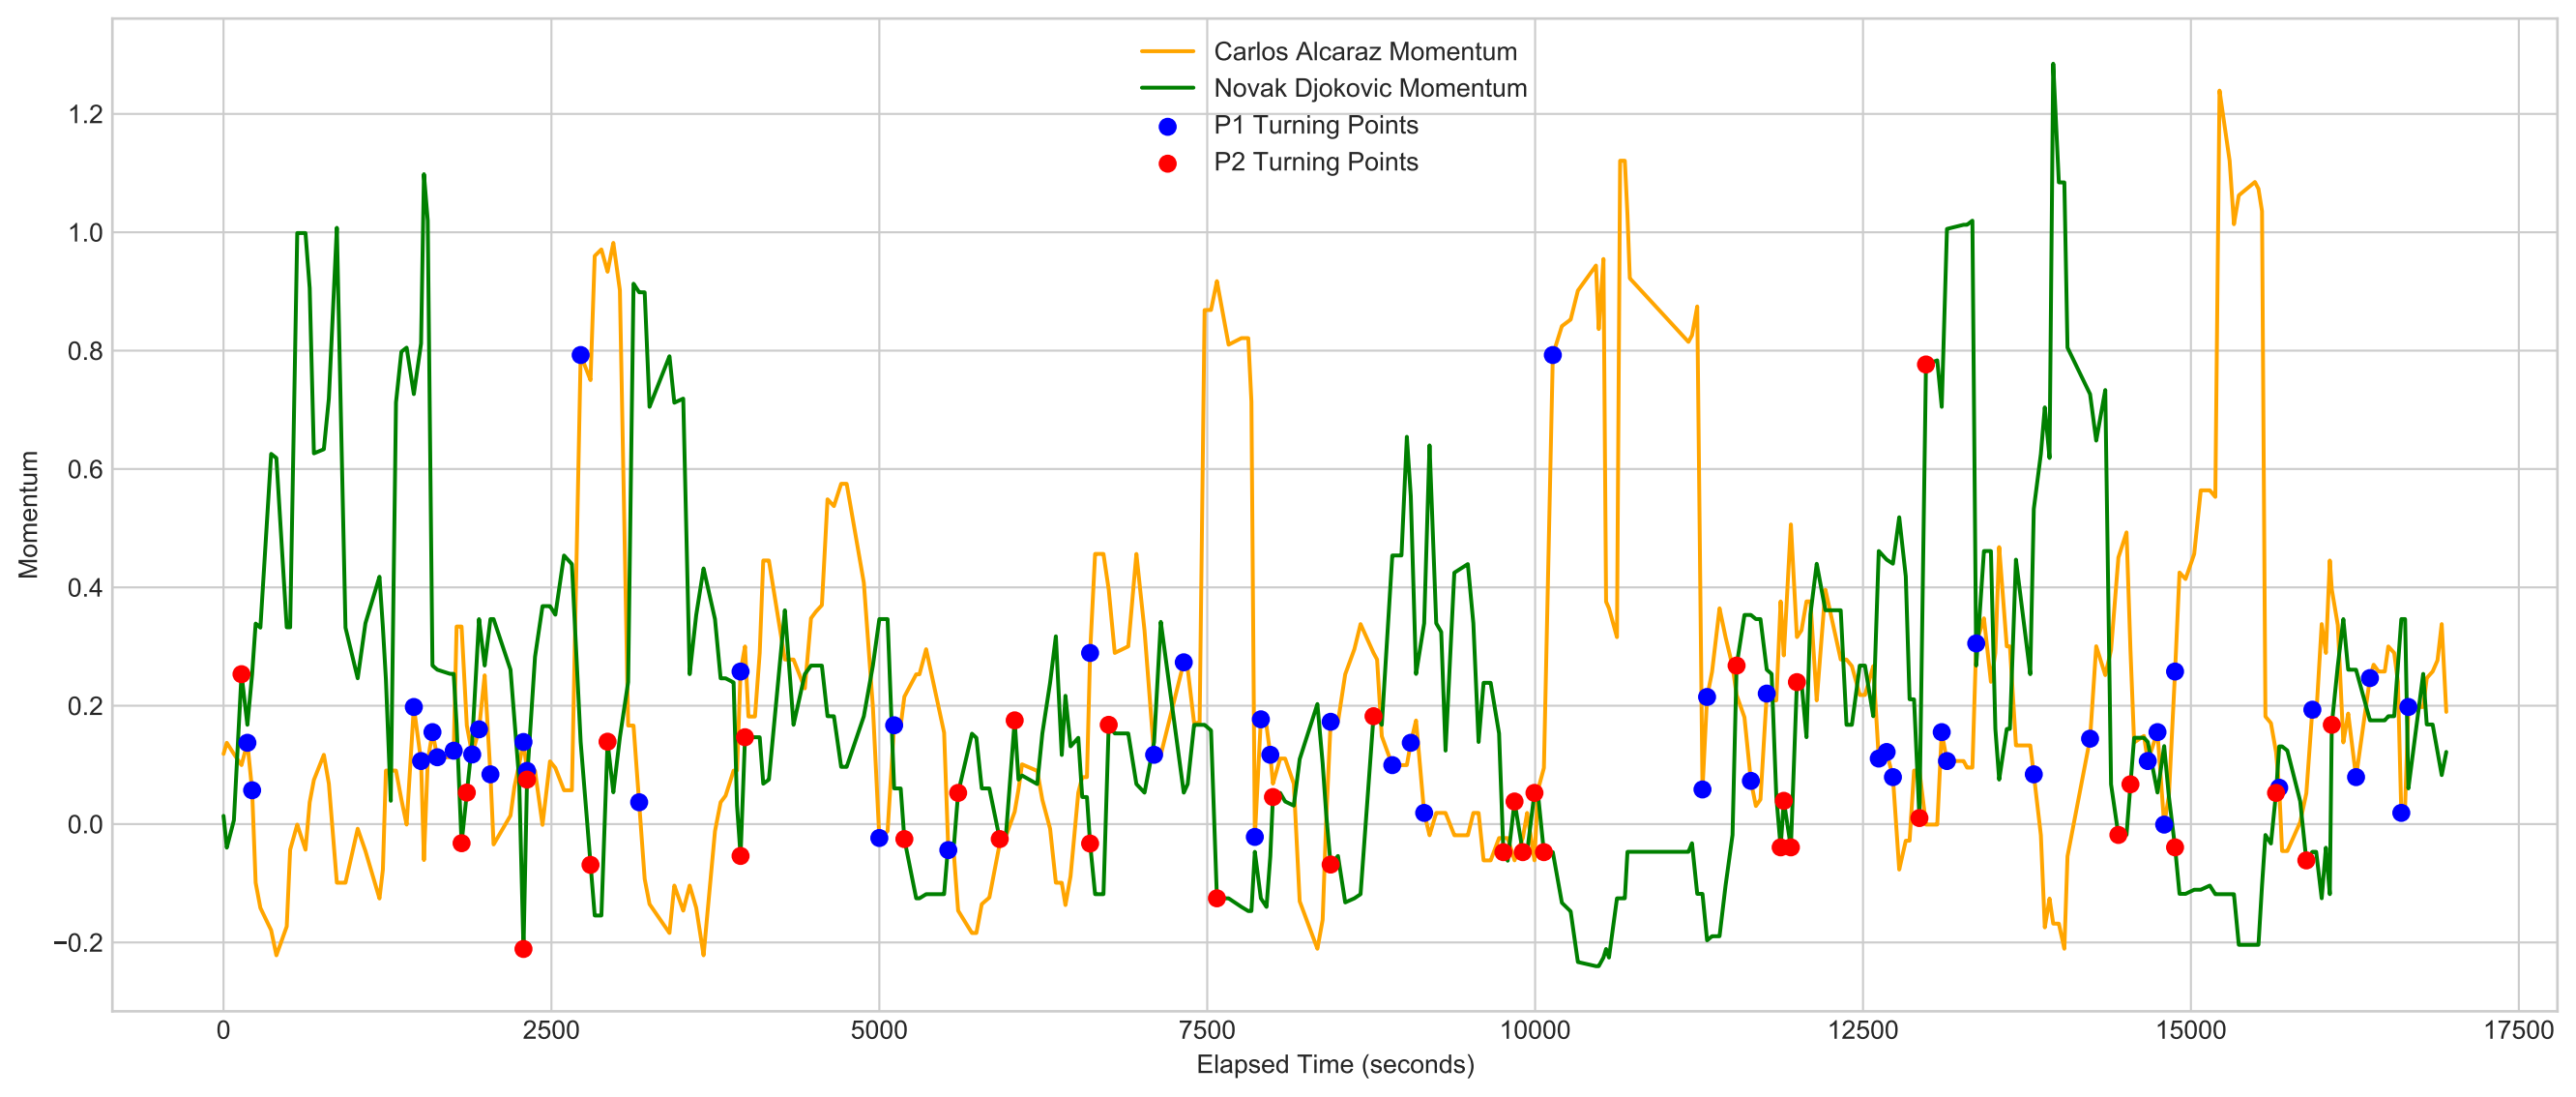
\includegraphics[scale=0.4]{figure//zzd.png}
	\caption{Momentum change and turning points}
	\label{zzd}
\end{figure}
Figure \ref{zzd} shows the momentum of players 1 and 2 fluctuating throughout the match. The marked turning points signify moments of significant momentum change, corresponding to the players' performance improvements and declines. This graph can assist coaches in identifying moments when the match shifts from one player to another, allowing for timely preparation of countermeasures.
%%聚类聚类

\subsection{Purification factor}

Aiming for players to exhibit better momentum and performance in matches, we introduce the concept of "Purification factor." These account for factors in matches that athletes may find difficult or impossible to adjust. Hence, "Evolutionary Indicators" refer to elements athletes can confidently adjust in a short timeframe. We prioritize factors that can be adjusted by athletes based on their correlation with momentum, performance, and turning points.
	\begin{itemize}
	\setlength{\parsep}{0ex} %段落间距
	\setlength{\topsep}{2ex} %列表到上下文的垂直距离
	\setlength{\itemsep}{1ex} %条目间距
	\item \textbf{Serve Advantage:} Reflects the advantage of the server over the receiver in terms of scoring and holding serve in tennis matches.
	
	\textbf{$\hookrightarrow$Suggestion:} Optimize technique and adjust tactics to enhance the quality of service, and use conservative tactics in critical games to ensure the stability of service holds.
	
	\item \textbf{Break Points Won:} Refers to winning a point in the opponent's service game, directly related to the ability to change the momentum of the match.
	
	\textbf{$\hookrightarrow$Suggestion:} Analyze the opponent's serving habits deeply, adjust tactics to improve the efficiency of breaking serve, and strengthen psychological training to enhance performance in critical moments.
	
	\item \textbf{Unforced Errors:} Errors made by a player under no pressure from the opponent, with a focus on reducing these mistakes to improve performance.
	
	\textbf{$\hookrightarrow$Suggestion:} Work with coaches to refine technical adjustments, and reduce error rates through psychological and technical training.
	
	\item \textbf{Winners:}  Points earned by the player through aggressive play, reflecting the ability to attack and proactively control the match.
	
	\textbf{$\hookrightarrow$Suggestion:} Intensify offensive tactical training, use tactical analysis to identify opponent weaknesses, and increase opportunities for winners.
	
	\item \textbf{ACE Won:} Specifically refers to scoring directly from the serve, without the need for rally exchange, demonstrating precision and power in the serve.
	
	\textbf{$\hookrightarrow$Suggestion:} Improve serving techniques, increase the number of aces, and use them to stabilize service games at crucial moments.
	
	\item \textbf{Double Fault:}  Refers to two consecutive serving errors, affecting the stability and confidence in the service game.
	
	\textbf{$\hookrightarrow$Suggestion:} Combine technical and psychological training to reduce the rate of double faults, and adopt conservative strategies in critical games to ensure stability.
	
\end{itemize}


By strategically improving certain indicators, players can significantly enhance their performance and maintain consistent momentum in the Wimbledon competition. These strategies need to be adaptable in practice, tailored to the specifics of each match and opponent for optimal results. Through comprehensive training and strategic planning, it's believed that players will achieve outstanding results at Wimbledon.



\section{GSRF Model Generality in Tennis Prediction}
Some common evaluation metrics used in machine learning algorithms for prediction include the Root Mean Square Error (RMSE) and the Mean Absolute Error (MAE). Specifically, MSE is the mean of the square differences between the predictions and the original data, while MAE is the mean of the absolute differences between the predictions and the original data. The formulas are as follows:

\begin{equation}
	\operatorname{RMSE}=\sqrt{\frac{1}{n} \sum_{i=1}^n\left(y_i-\hat{y}_i\right)^2}
\end{equation}

\begin{equation}
	\mathrm{MAE}=\frac{1}{n} \sum_{i=1}^n\left|y_i-\hat{y}_i\right|
\end{equation}
where $n$ is the number of observation, $y_i$ is the $i$-th actual observed value, $\hat{y}_i$ is the $i$-th predicted value.





\begin{table}[ht]
	\centering
	\begin{tabular}{lcccc}
		\hline
		\rowcolor{green!30}
		{Model} & {RMSE} & {MAE} & {MAPE} & {$R^2$} \\
		\hline
		\rowcolor{yellow!30}
		GSRF & 0.4712 & 0.3875 & 0.3258 & 0.9853 \\
		\rowcolor{yellow!30}
		GRFA & 0.9871 & 0.9412 & 1.218 & 0.8951 \\
		\hline
	\end{tabular}
	\caption{Model performance comparison.}
	\label{table:model_performance}
\end{table}

Based on the data in the table above, the GSRF prediction model has very good predictive performance for future momentum differences fluctuations. With an RMSE of 0.4712, and an MAE of 0.3875, this indicates that the model can predict the fluctuations of momentum differences in the future based on past fluctuations in players' momentum differences 	\cite{sipko2015machine} . This demonstrates the effectiveness of the GSRF algorithm in predicting momentum fluctuations. \\ 

In addition, we looked for the2023 women's tennis match data on the official Wimbledon website, used the data before the finals to train the model, and then predicted the fluctuations in the players' momentum differences during the finals as shown in Figure \ref{sl3}.

\begin{figure}[H]
	\centering
	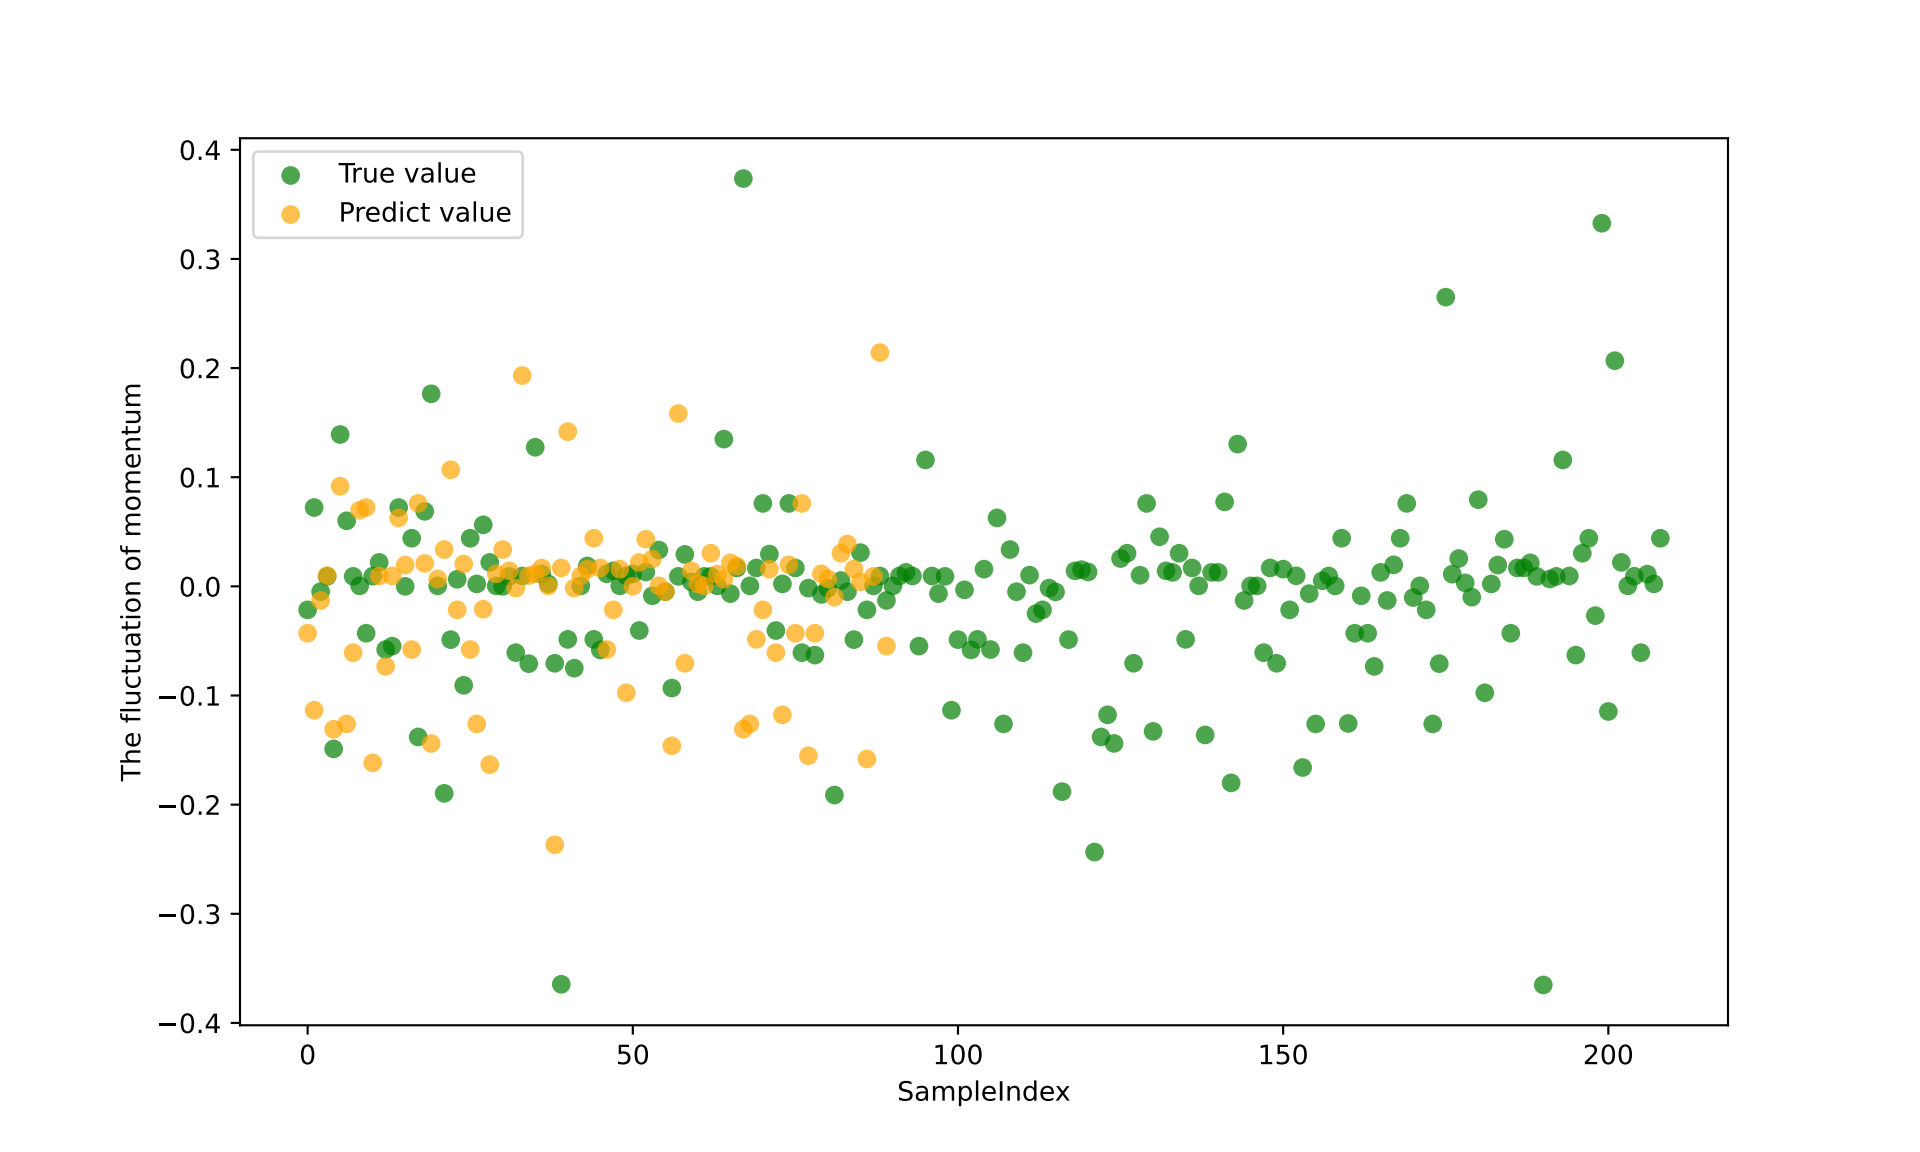
\includegraphics[scale=0.56]{figure//sl3.png}
	\caption{Model performance comparison}
	\label{sl3}
\end{figure}
The distribution of the scatter plot in the figure shows that the predicted results are largely concentrated around the value of 0, indicating that the GSRF model has a good prediction effect on the women's matches.

\section{Sensitivity Analysis and Robustness Analysis}

\subsection{Sensitivity Analysis}
We conducted a sensitivity analysis on the input parameters of the GSRF prediction model to test its sensitivity to changes in input parameters when predicting match fluctuations, as shown in Figure \ref{mg1}.

\begin{figure}[H]
	\centering
	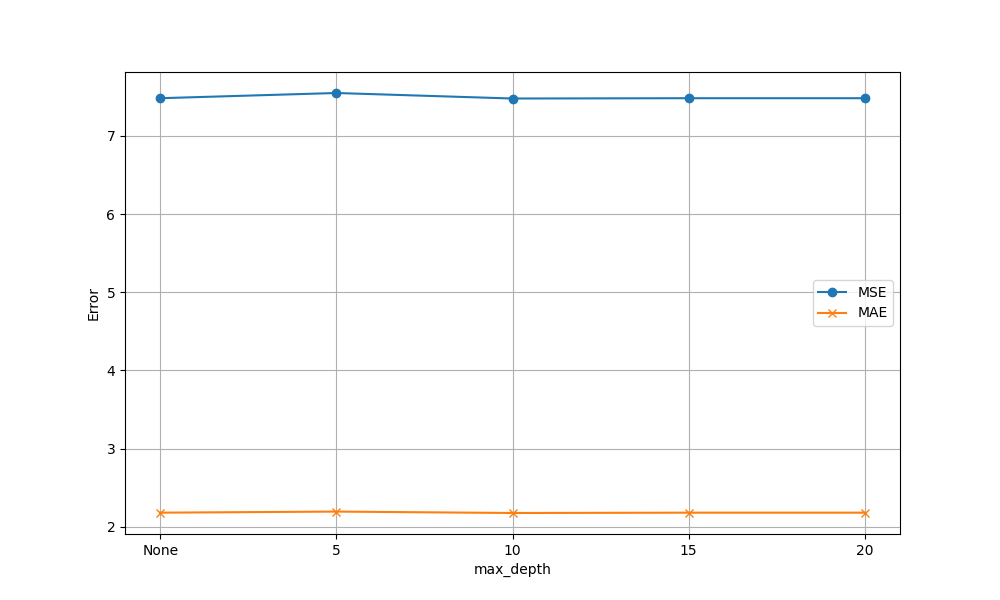
\includegraphics[scale=0.63]{figure//mg1.png}
	\caption{Sensitivity of p1$\_$net$\_$pt$\_$won}
	\label{mg1}
\end{figure}

The Figure shows that variations in max$\_$depth have minimal impact on model performance, suggesting that the GSRF prediction model has low sensitivity to changes in p1$\_$net$\_$won, indicating high stability.

\subsection{Robustness Analysis}
We added Gaussian noise to the model's input parameters to assess its stability. The Gaussian noise formula is as follows: 

\begin{equation}
	w_j=\frac{d_j}{\sum_{j=1}^m d_j}, j=1, \ldots, m
\end{equation}

where $x$ represents the amplitude of a random signal, $\mu$ represents the mean, and $\sigma$ represents the standard deviation. 
\clearpage
The result of robustness analysis is show in Figure \ref{mg2}.
\begin{figure}[H]
	\centering
	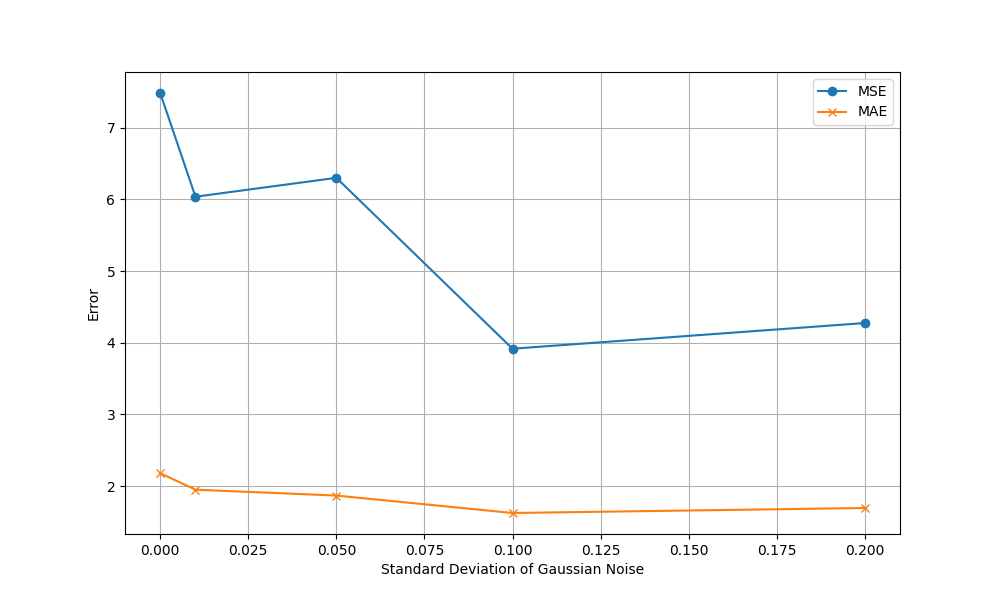
\includegraphics[scale=0.63]{figure//mg2.png}
	\caption{Model robustness to gaussian noise}
	\label{mg2}
\end{figure}
It shows that our model maintains stable performance under low levels of Gaussian noise. However, as noise levels increase, the model's error rises. This indicates the model has some robustness to minor data disturbances, but its accuracy is affected by significant declines in data quality.











	
	\section{Strengths and Weaknesses}
	\noindent{\large\textbf{Strengths:}}
	\vspace{0.3cm}
	\begin{itemize}
		\item A Degree of Versatility: Demonstrating the effectiveness of the GSRF model in various scenarios, including men's and women's matches at Wimbledon.
		\item Performance Evaluation: Applying RMSE, MAE, and MAPE as evaluation metrics and conducting sensitivity analyses ensures a comprehensive assessment of model accuracy and robustness.
		\item Comprehensive Analysis: Utilizing PCA for dimensionality reduction and WME entropy weighting for weight allocation, it demonstrates an orderly method of quantifying performance.
		\item Performance Evaluation: Applying RMSE, MAE, and MAPE as evaluation metrics and conducting sensitivity analyses ensures a comprehensive assessment of model accuracy and robustness.
	\end{itemize}
	\vspace{0.3cm}
	{\large\textbf{Weaknesses:}}
	\vspace{0.3cm}
	\begin{itemize}
		\item Subjectivity in Weight Allocation: Although the WME entropy method provides a systematic approach, the initial selection of variables for the model may still introduce subjectivity.
		\item Applicability in Certain Scenarios Needs Verification: The model was built using Wimbledon data, and its applicability to other non-Wimbledon events remains to be verified, considering factors such as the playing surface.
	\end{itemize}




	
	
	
	
	\newpage
	
	% 以下为信件/备忘录部分,不需要可自行去掉
	% 如有需要可将整个 letter 环境移动到文章开头或中间
	% 请在后一个花括号内填写信件(Letter)或备忘录(Memorandum)标题
	%审视艺术家和流派的进化和革命趋势
	
	\begin{letter}{Memo}
		\begin{flushleft}  % 左对齐环境,无首行缩进
			\noindent\rule{\textwidth}{1pt}
			
			\vspace{-0.1cm}
			
			\noindent \ To: Coaches
			
			\vspace{-0.1cm}
			
			\noindent \ From: Team \#2409859
			
			\vspace{-0.1cm}
			
			\noindent \ Date: February 5, 2024
			
			\vspace{-0.2cm}
			
			\noindent\rule{\textwidth}{1pt}
			
			
		\end{flushleft}
		
Recently, we have completed an in-depth analysis of the men's singles matches at the 2023 Wimbledon Tennis Championships. We hope that the insights and strategies provided by these data can help you and your players achieve better results in future competitions.

By comprehensively applying PCA (Principal Component Analysis), WME (Weighted Mean Entropy method), Run Test Algorithm, GSRF (Generalized Spectral Random Field) and GRFA (Generalized Random Field Algorithm) models, and the CUMSUM (Cumulative Sum Control Chart) algorithm, we have highlighted the significant impact of our analytical methods on tennis coaching and performance strategy transformation. Our extensive application of PCA, WME entropy weights, Run Test Algorithm, GSRF, GRFA models, and CUMSUM algorithm underscores the critical role of data-driven insights in sports analytics. This research demonstrates the potential to significantly enhance training methodologies and competitive strategies through the strategic application of predictive modeling and performance analysis.

Our team is committed to ongoing dialogue to explore how these insights can be effectively translated into competitive advantages during matches. Stakeholders can also refer to the "performance factors" directly provided in our paper to train athletes more intuitively, including improving service advantages, increasing breakpoints, reducing unforced errors, enhancing the number of winners and aces, and reducing double faults. You should help players optimize these adjustable factors through technical training, psychological preparation, and tactical analysis. It is advised that players engage in regular service practice, with a particular focus on performance under match pressure, to improve stability and competitiveness during matches. By integrating these recommendations, players can gain better momentum and exhibit outstanding performance in competition.

We strongly recommend you integrate the findings of this study into their preparation and tactical approaches, especially by leveraging the predictive accuracy of the GSRF model to understand momentum shifts and identify key moments in matches. Moreover, coaching teams need to receive regular data analysis training to proficiently use these advanced tools for strategic planning and performance optimization.



We sincerely hope that the above analysis can offer you new perspectives and strategies to help your players perform better in upcoming matches. If you have any questions or require further information, we are more than willing to assist. Thank you for your trust in our work, and we look forward to further collaboration with you.
		
		
		% \cite{huttoVADERParsimoniousRuleBased2014}
		
		\hfill Yours Sincerely,
		
		\hfill Team $\#$2409859  
	\end{letter}
	
	\clearpage
	
	
	\bibliographystyle{plain}
	\bibliography{wenxian}
	\clearpage
	

	\appendix
	\centering
	\section*{Report of Use AI}
	\addcontentsline{toc}{section}{Report of Use AI}
	\thispagestyle{empty}
	
	
	\begin{table}[!ht]
		\centering
		\begin{tabular}{|p{17cm}|}
			\hline 	    \rowcolor{black!8}
			Query1:\\ \rowcolor{black!8}
			What is unforced error in tennis? \\
			\hline
		\end{tabular}
		\begin{tabular}{|p{17cm}|}
			Output1:\\
			A unforced error in tennis refers to a mistake made by a player under no immediate pressure from the opponent's shot, leading to the loss of a point. It occurs when a player fails to return the ball in the court without being forced into a difficult position by an opponent's aggressive play. Non-forced errors typically result from poor shot selection, lack of concentration, or technical mishaps, contrasting with forced errors, which are caused by the opponent's skillful play.
			\\
			\hline
		\end{tabular}
		%%第二个	
		\begin{tabular}{|p{17cm}|}
			\hline  \rowcolor{black!8}
			Query2:\\  \rowcolor{black!8}
			What does ace mean in tennis? \\
			\hline
		\end{tabular}
		\begin{tabular}{|p{17cm}|}
			Output2:\\
			In tennis, an ace occurs when a player serves the ball so effectively that the opponent cannot touch it with their racket, resulting in an immediate point for the server. Aces are a powerful tool in a player's arsenal, showcasing both precision and speed in serving.
			\\
			\hline
		\end{tabular}
		%%第三个
		\begin{tabular}{|p{17cm}|}
			\hline  \rowcolor{black!8}
			Query3:\\  \rowcolor{black!8}
			Summarize Our Titles:
			
			1. **Quantitative Assessment of Player Performance Using PCA and WME Entropy Weighting Method**
			
			2. **Analysis of Momentum Volatility in Tennis Matches Using Run Test**
			3. **Predicting Momentum Fluctuations in Tennis Matches with the GSRF Model**
			4. **Validation of the GSRF Model's Generality in Tennis Match Prediction** \\
			\hline
		\end{tabular}
		\begin{tabular}{|p{17cm}|}
			Output3:\\
			1. **Player Performance Quantification with PCA \& WME**
			
			2. **Tennis Momentum Volatility via Run Test**
			
			3. **GSRF Model for Tennis Momentum Prediction**
			
			4. **GSRF Model Generality in Tennis Prediction**  \\
			
			\hline
		\end{tabular}

	
	
	
	\end{table}
	
\thispagestyle{empty}
	
		\begin{table}[!ht]
		\centering

		\begin{tabular}{|p{17cm}|}
			\hline
			Output3:\\
			1. **Player Performance Quantification with PCA \& WME**
			
			2. **Tennis Momentum Volatility via Run Test**
			
			3. **GSRF Model for Tennis Momentum Prediction**
			
			4. **GSRF Model Generality in Tennis Prediction**  \\
			
			\hline
		\end{tabular}
		\begin{tabular}{|p{17cm}|}
			\hline  \rowcolor{black!8}
			Query4:\\  \rowcolor{black!8}
			I want to know some papers and documents about tennis competition. Please recommend some links to me \\
			\hline
		\end{tabular}
		\begin{tabular}{|p{17cm}|}
			Output5:\\
			I've found some fascinating research on tennis matches that spans various aspects of the game, including the impact of sleep and match timing on performance, the use of technology for analyzing wheelchair tennis, predictive modeling of match outcomes, and the application of artificial intelligence for tracking game metrics. These papers delve into how sleep behavior affects players, employ inertial measurement units to assess performance in wheelchair tennis, utilize the Glicko model and Monte Carlo simulations for predictions, and explore AI for recording ball passes over the net.
			For more in-depth exploration, please visit: https://typeset.io/search?q=tennis matches
			Feel free to ask more questions if you need additional insights or have other topics of interest!  \\
			
			\hline
		\end{tabular}
		
		\begin{tabular}{|p{17cm}|}
			\hline  \rowcolor{black!8}
			Query5:\\  \rowcolor{black!8}
			I want to find Wimbledon 2023 Women's Singles Championship data \\
			\hline
		\end{tabular}
		\begin{tabular}{|p{17cm}|}
			Output3:\\
			It seems there are no direct academic papers or publications specifically detailing the Wimbledon 2023 Women's Singles Championship data in the searched database. The search results did not yield relevant documents related to sports results or detailed analyses of specific tournaments such as Wimbledon 2023.
			For more comprehensive and detailed search results, you might want to explore sports databases, official Wimbledon websites, or sports a  \\
			
			\hline
		\end{tabular}
		
		
		
		
	\end{table}
	
	
	
	
	
\end{document}